\chapter{Towards Best-Performed Query Term Selection}
\label{cha:analysis}
In this chapter, we mainly focus on recognizing the reasons why standard IR methods fail when the relevant patent documents are complete and in English. In fact, we will investigate the problem from term analysis point of view for both patent query and relevant documents because we are interested in finding what is wrong in term matching process between a patent query and relevant patents. 

%%%%%%%%%%%%%%%%%%%%%%%%%%%%%%%%%%%%%%%%%%%%%%%%%%%%%%%%%%%%%%
%%%%%%%%%%%%%%%%%%%%%%%% SECTION 1 %%%%%%%%%%%%%%%%%%%%%%%%%%
%%%%%%%%%%%%%%%%%%%%%%%%%%%%%%%%%%%%%%%%%%%%%%%%%%%%%%%%%%%%%%

\section{Term Mismatch}
\label{sec:termmismatch}
%\input{TermAnalysis/termmismatch}
Standard retrieval models rank documents based on term matching between the query and documents.  
A significant term mismatch between the query patent and relevant patents has been mentioned the
main cause for low effective patent prior art search in previous works~\citep{roda2010clef}~\citep{magdy2012toward}. 
We examine term overlap between Patent Query and three different patent documents: (i) retrieved relevant patents (TPs), (ii) retrieved non-relevant patents (FPs), and (iii) non-retrieved relevant patents (FNs), respectively, by calculating the average term overlap per query as follows:
%%%%%%%%%%%%%%%%%%%%%%%%%%%%%%%%%%%%%%%%%%%%%%%%%%%%%%%%%%%%%%
\begin{equation} 
TO (Q) = \frac{1}{|D|}\sum_{d\in D}\frac{|terms_{Q\cap d}|}{|Q|}
\label{eq:fntermoverlap}
\end{equation}
%\vspace*{-1ex}
%\begin{displaymath}t\in \lbrace \mbox{terms in top-100 retrieved documents}\rbrace\end{displaymath}
%%%%%%%%%%%%%%%%%%%%%%%%%%%%%%%%%%%%%%%%%%%%%%%%%%%%%%%%%%%%%%

where $TO(Q)$ is the average term overlap per query --- we calculate this score for TP, FP, and FN patents respectively, $D$ is a collection of TP patents, FP patents, or FN patents for each query respectively, $|D|$ is the number of TP patents, FP patents, or FN patents for each query, $ |terms_{Q\cap d}| $ is the number of query terms appear in each TP, FP, or FN patent, $ |Q| $ is the size of the query.

The results has been illustrated in Figure~\ref{fig:overlap}. We conclude two main facts:
\begin{enumerate}
\item For the majority of queries (around 94\% of queries), patent documents are retrieved (TPs and FPs) when they have a term overlap with a query above $ 0.2 $.
\item We can also see sufficient term overlap with the query for FN patents, whereas, compared to TPs and FPs, more queries can be seen with the term overlap less than $ 0.2 $ (about 24\% of queries). 
\end{enumerate}
 
%%%%%%%%%%%%%%%%%%%%%%%%%%%%%%%%%%%%%%%%%%%%%%%%%%%%%%%%%%%%%%
\begin{figure}[t!]
\begin{centering}
\subfigure[Query and TP patents.]{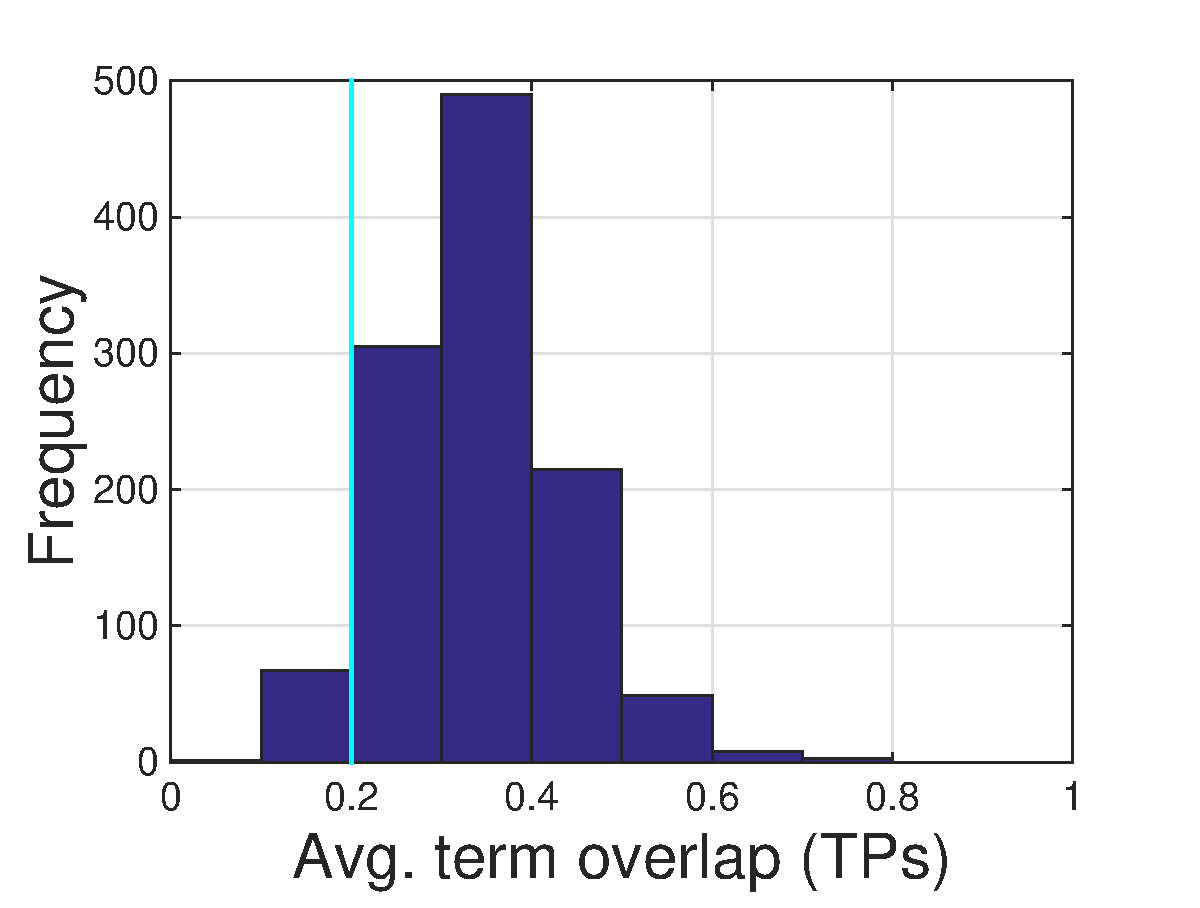
\includegraphics[width=5cm]{figs/to-tps.eps}}\subfigure[Query and FP patents.]{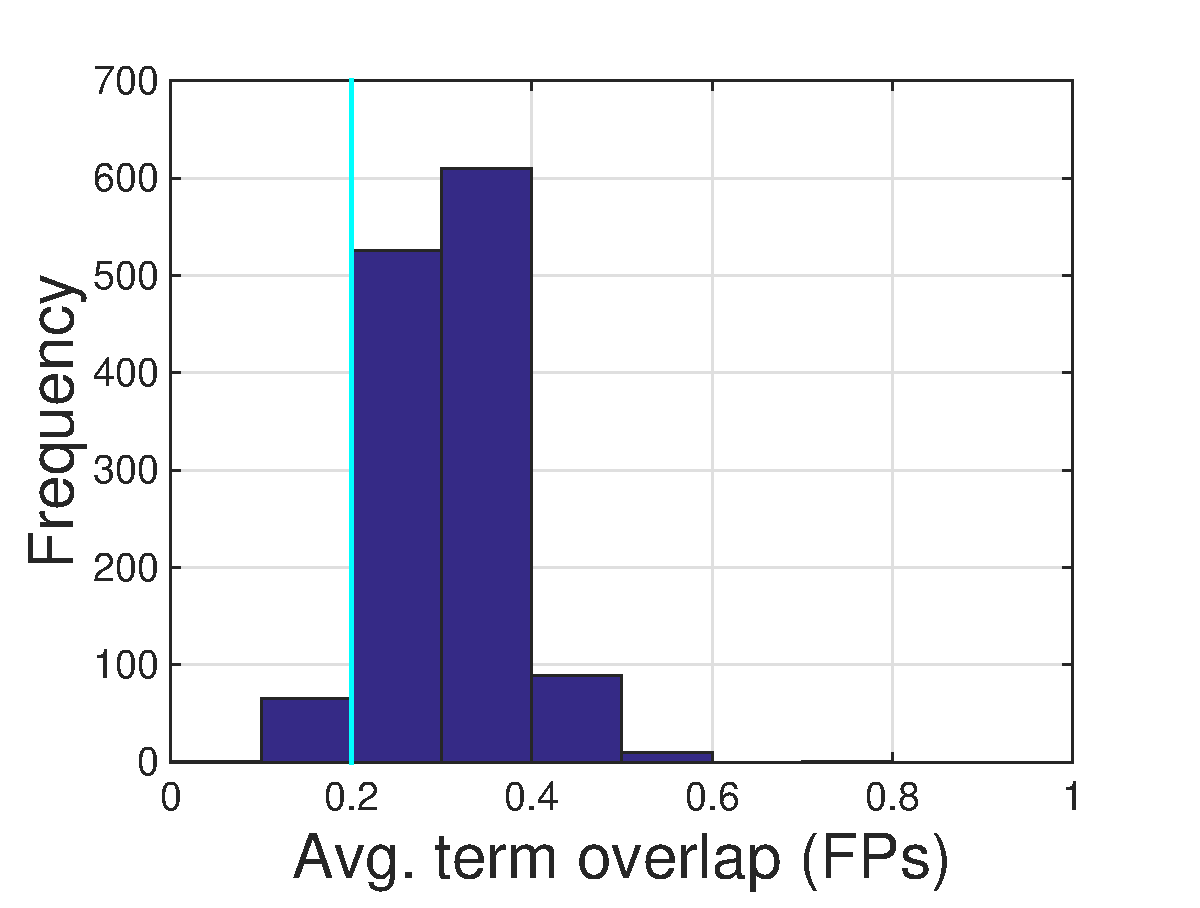
\includegraphics[width=5cm]{figs/to-fps.eps}}\subfigure[{Query and FN patents.}]{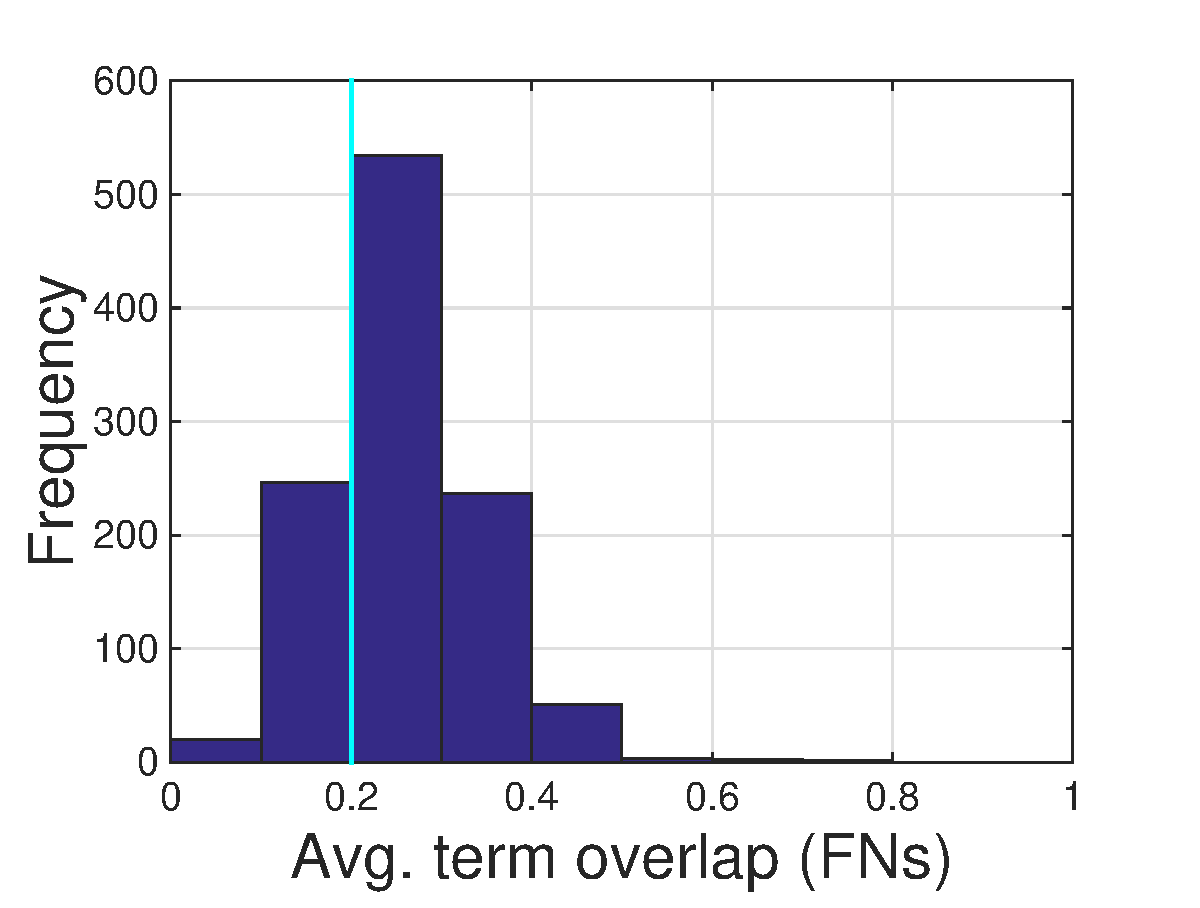
\includegraphics[width=5cm]{figs/to-fns.eps}}
\par\end{centering}

\protect\caption{The distribution of term overlap between the query and documents over 1303 test queries.}
\label{fig:overlap}
\end{figure}
%%%%%%%%%%%%%%%%%%%%%%%%%%%%%%%%%%%%%%%%%%%%%%%%%%%%%%%%%%%%%%
In summary, this experiment shows that low or zero term match is not the main cause of low effectiveness for patent prior art search.
%%%%%%%%%%%%%%%%%%%%%%%%%%%%%%%%%%%%%%%%%%%%%%%%%%%%%%%%%%%%%%
%%%%%%%%%%%%%%%%%%%%%%%%% SECTION 2 %%%%%%%%%%%%%%%%%%%%%%%%%%
%%%%%%%%%%%%%%%%%%%%%%%%%%%%%%%%%%%%%%%%%%%%%%%%%%%%%%%%%%%%%%
\section{Oracular Relevance Feedback System}
\label{sec:oraculrquery}
A query is optimal if it ranks all relevant documents before
those that are not relevant, that is, it would lead to a ranking with an average precision of 1.0. A query
is most likely to achieve a ranking that is as close to optimal as possible if it contains all terms that
appear in all relevant documents, but explicitly discounts all terms that occur in non-relevant documents~\citep{manning2008introduction}.
Inspired by this fact, we develop an oracular relevance feedback system, which
extracts terms from the judged relevant documents to derive an upper bound on performance of
standard Okapi BM25 and Language Models (LM) retrieval
algorithms for patent prior art search.
%\subsection{Oracular Term Selection}
\subsection{Scoring Terms}
\label{OracularTermSelection}
We aim at identifying terms, which are considered useful for the query to get the best retrieval effectiveness. For this purpose, 
after an initial run of reference Patent Query, we
calculate an Oracular Relevance Feedback ($\mathit{RF}$) score for each term in the top-100
retrieved documents as follows:
%%%%%%%%%%%%%%%%%%%%%%%%%%%%%%%%%%%%%%%%%%%%%%%%%%%%%%%%%%%%%%
\begin{equation}
RF(t,Q)=Rel(t)-Irr(t) 
 \label{eq:score}
\end{equation}
\begin{displaymath}t\in \lbrace \mbox{terms in top-100 retrieved documents}\rbrace\end{displaymath}
%%%%%%%%%%%%%%%%%%%%%%%%%%%%%%%%%%%%%%%%%%%%%%%%%%%%%%%%%%%%%%
where $ \mathit{Rel(t)} $ is the average term frequency in retrieved relevant patents and $ \mathit{Irr(t)} $ is the average term frequency in retrieved irrelevant patents. We assume words with a positive score are Useful Words since they are more frequent in relevant patents, while words with a negative score are Noisy Words as they appear more frequently in irrelevant patents. 

First, we seek for a pattern between the performance and the existence of \textit{useful words} for each query. We use different criteria to select the useful terms:
\begin{enumerate}
\item terms with positive scores(>0).
\item terms with the score higher than the positive median score.
\item terms with the score higher than a constant: 1, 5, and 10.
\item top-100 high-scored terms.
\end{enumerate}

The results have been shown in Figures~\ref{fig:overlap-r} and~\ref{fig:overlap-p}. 
%%%%%%%%%%%%%%%%%%%%%%%%%%%%%%%%%%%%%%%%%%%%%%%%%%%%%%%%%%%%%%
\begin{figure}[t!]
\begin{centering}
\subfigure[Useful Terms: $ \{t|RF(t, Q)>0\} $]{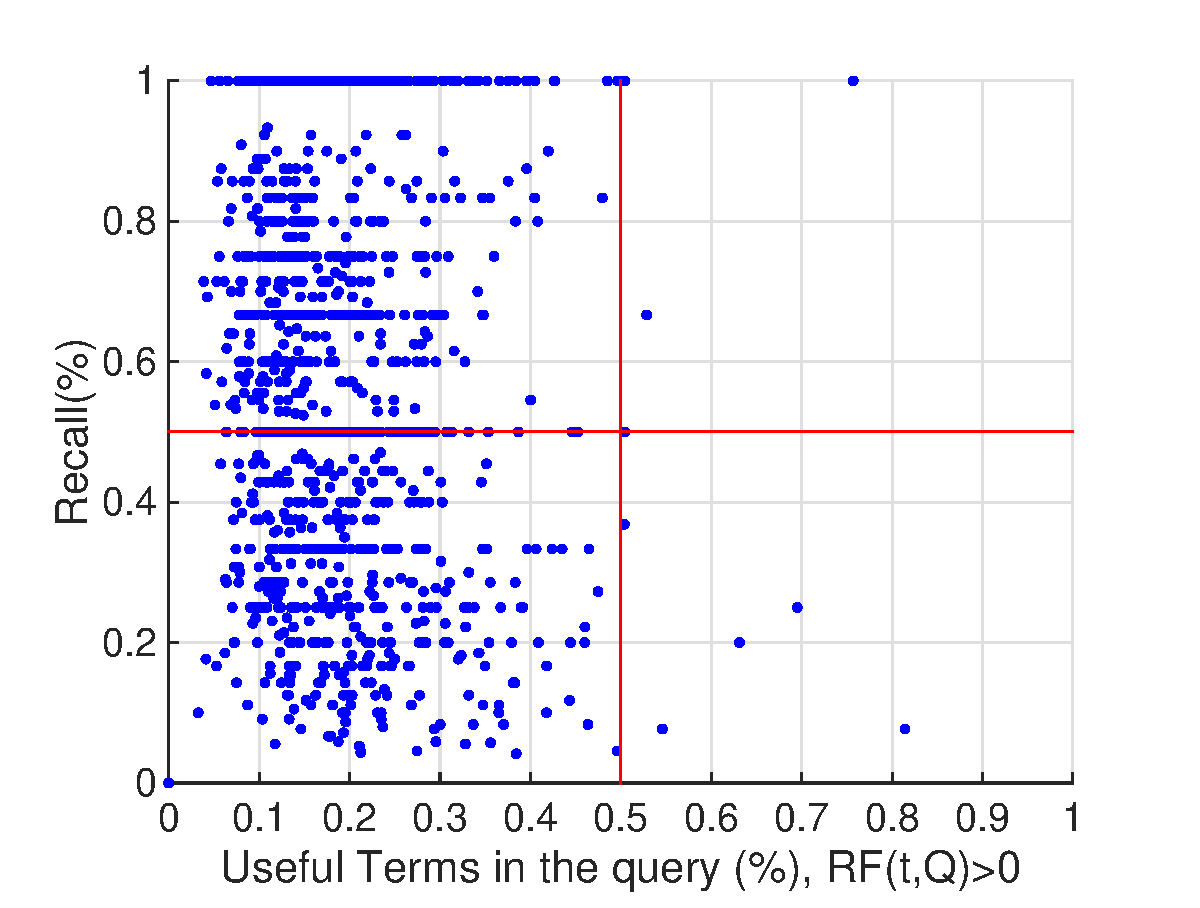
\includegraphics[width=5cm]{figs/greaterthan0-r.eps}} \hspace*{1.5cm} \subfigure[Useful Terms: $ \{t|RF(t, Q)>RF(t_{+median})\} $]{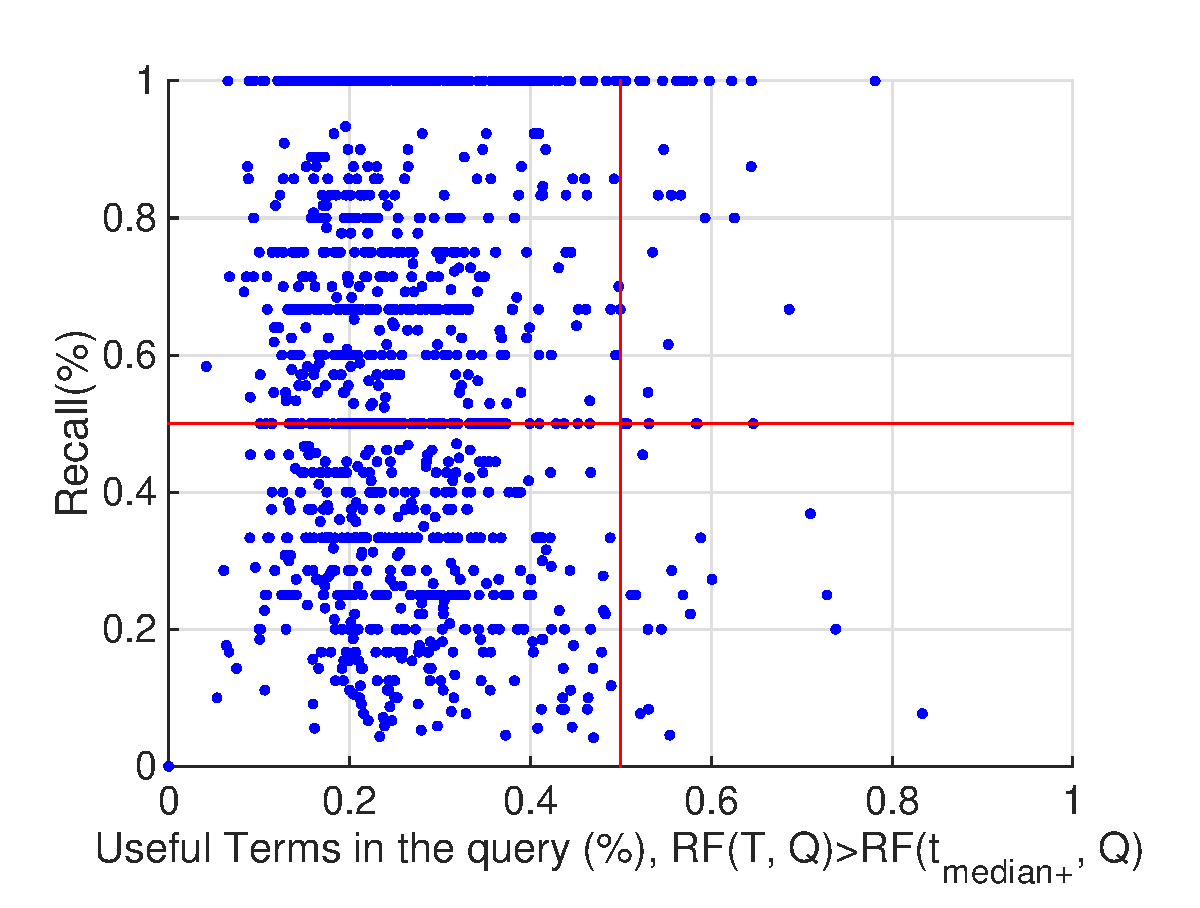
\includegraphics[width=5cm]{figs/greaterthanmedian-r.eps}}\\ \subfigure[{Useful Terms: $ \{t|RF(t, Q)>1 \}$}]{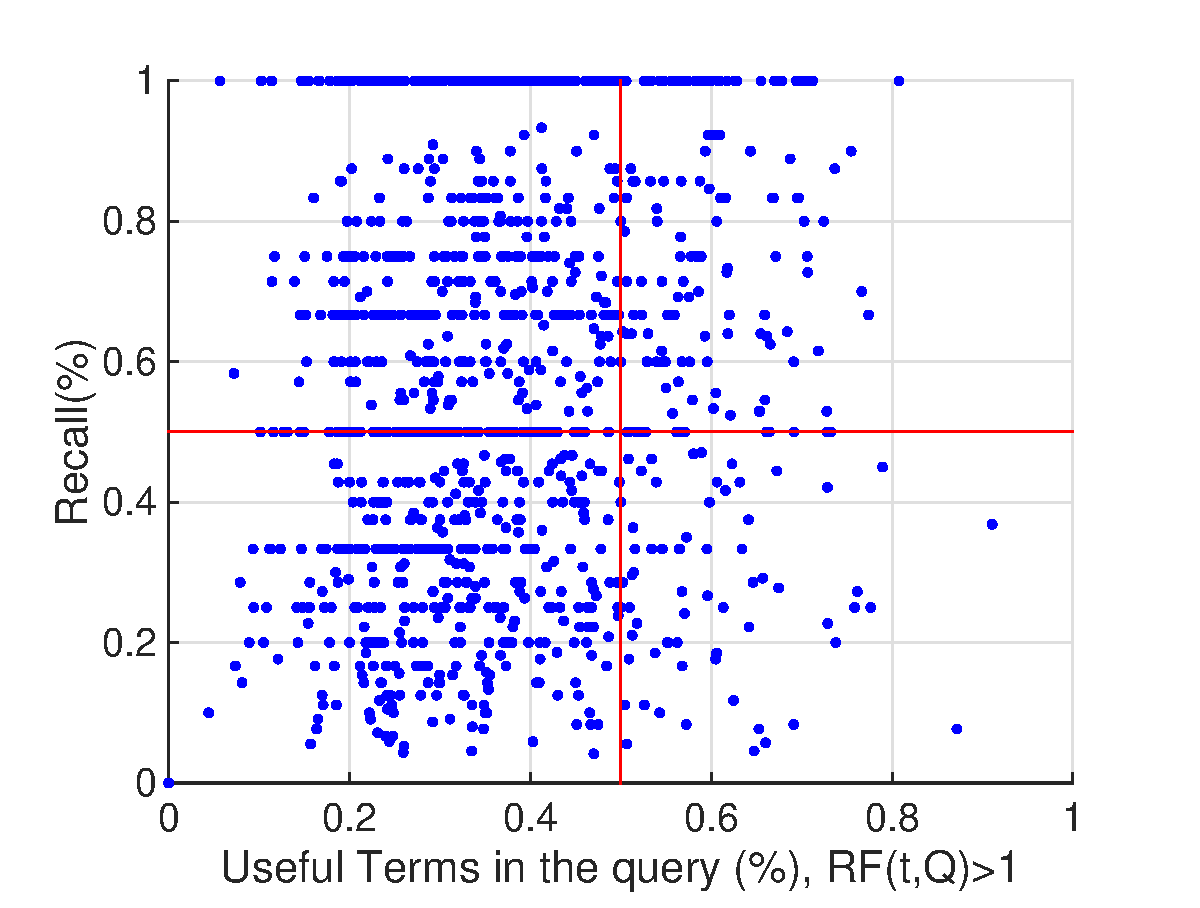
\includegraphics[width=5cm]{figs/greaterthan1-r.eps}} \hspace*{1.5cm} \subfigure[{Useful Terms: top 100 high-scored terms}]{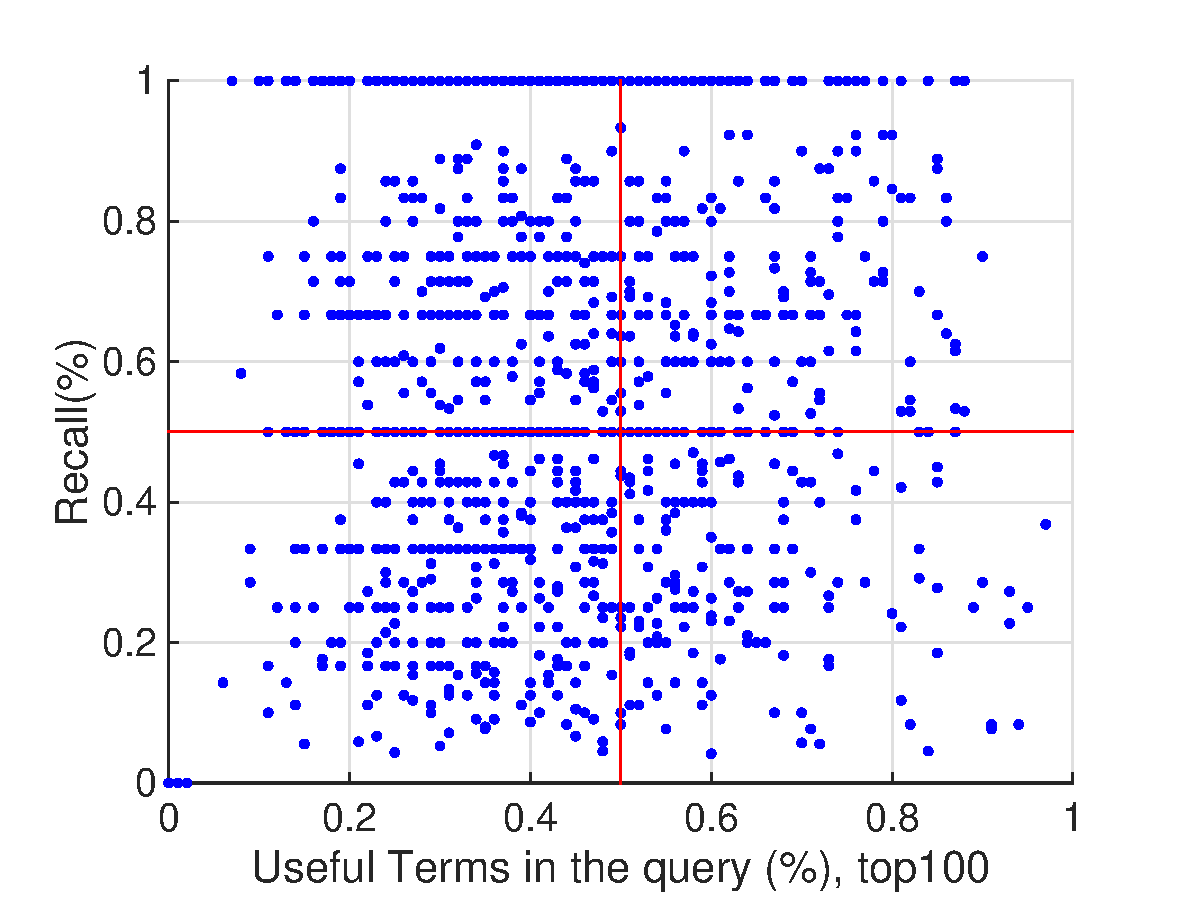
\includegraphics[width=5cm]{figs/top100-r.eps}}\\ \subfigure[{Useful Terms:$ \{t|RF(t,Q)>5 \}$}]{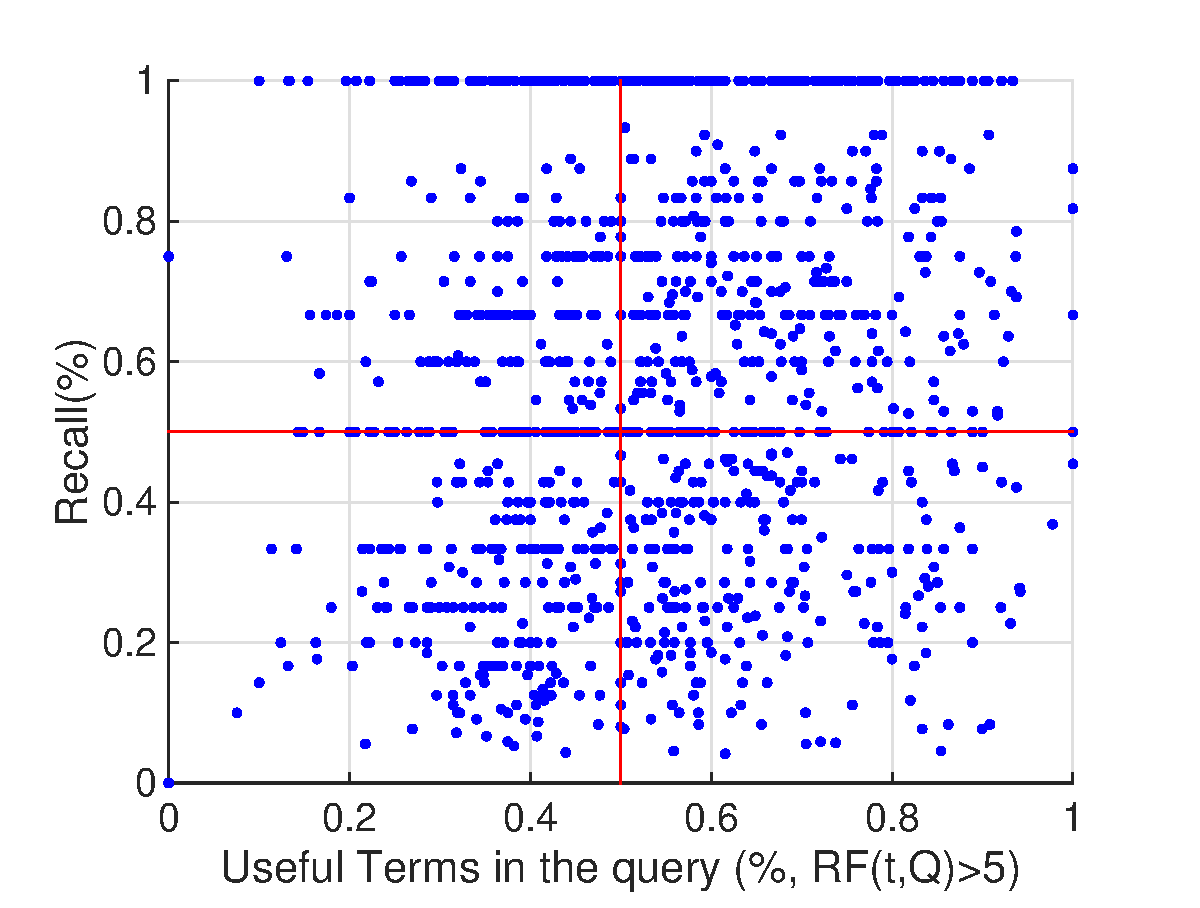
\includegraphics[width=5cm]{figs/greaterthan5-r.eps}} \hspace*{1.5cm} \subfigure[{Useful Terms: $ \{t|RF(t, Q)>10\} $}]{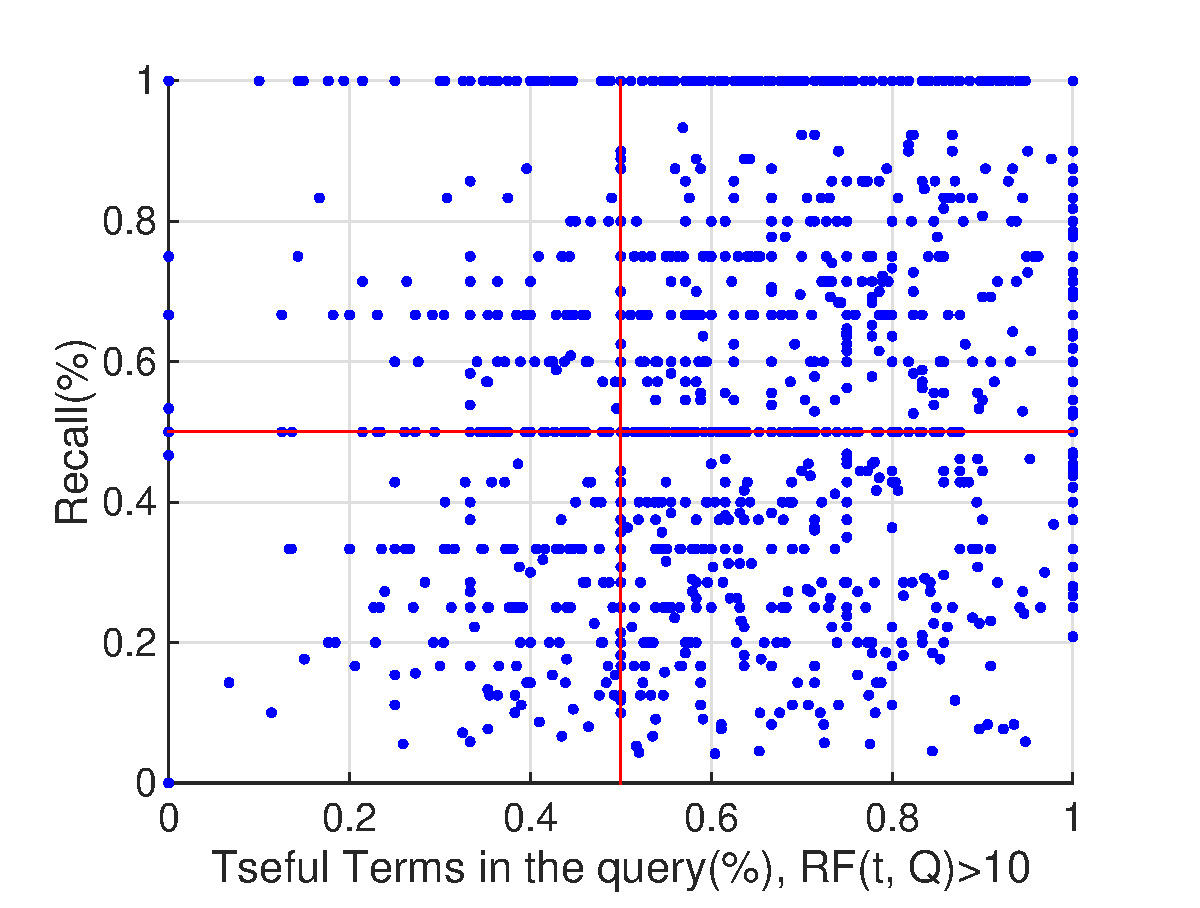
\includegraphics[width=5cm]{figs/greaterthan10-r.eps}}
\par\end{centering}

\protect\caption{Scatter plot of Recall vs. the overlap between useful terms and the the query.}
\label{fig:overlap-r}
\end{figure}
%%%%%%%%%%%%%%%%%%%%%%%%%%%%%%%%%%%%%%%%%%%%%%%%%%%%%%%%%%%%%%
%%%%%%%%%%%%%%%%%%%%%%%%%%%%%%%%%%%%%%%%%%%%%%%%%%%%%%%%%%%%%%
\begin{figure}[t!]
\begin{centering}
\subfigure[Useful terms: $ \{t|RF(t, Q)>0\} $]{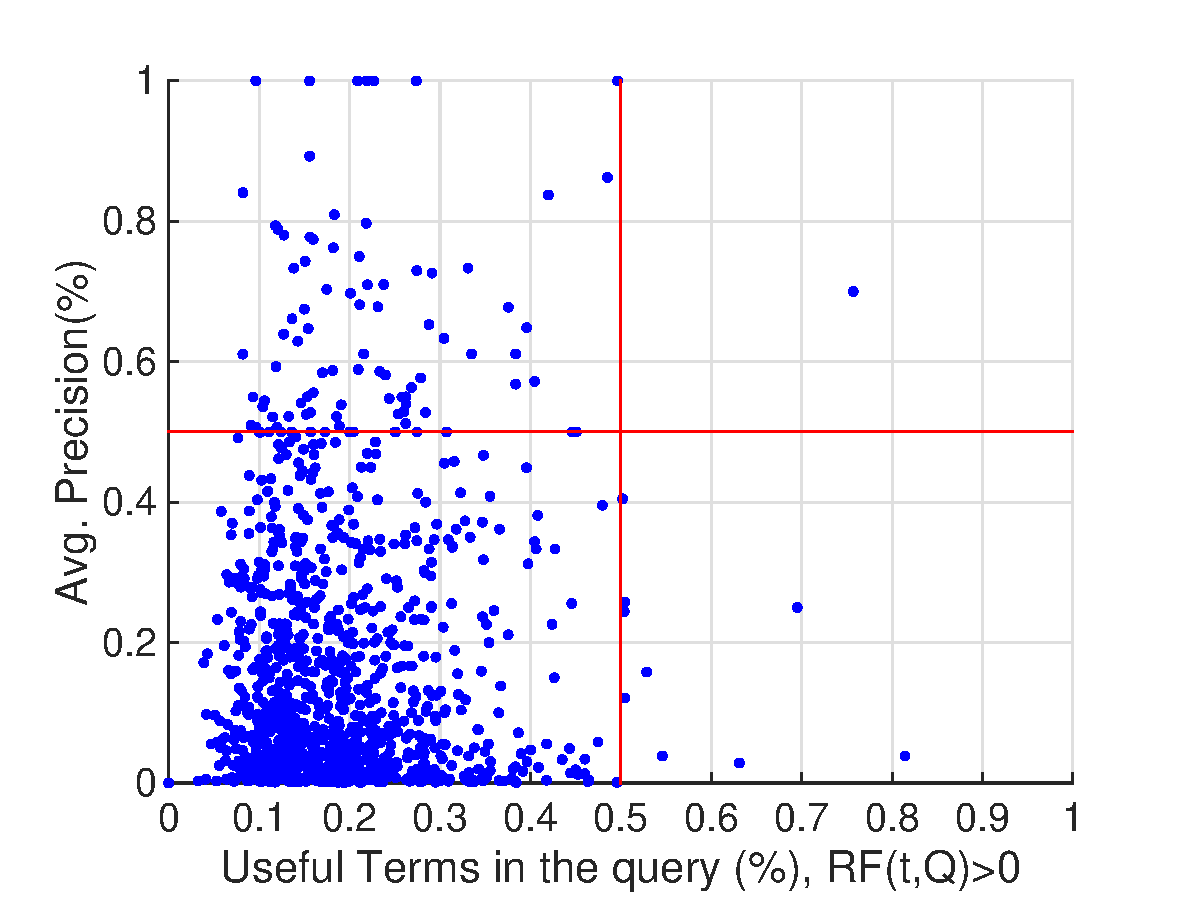
\includegraphics[width=5cm]{figs/greaterthan0-p}} \hspace*{1.5cm} \subfigure[Useful terms: $ \{t|RF(t, Q)>RF(t_{+median})\} $]{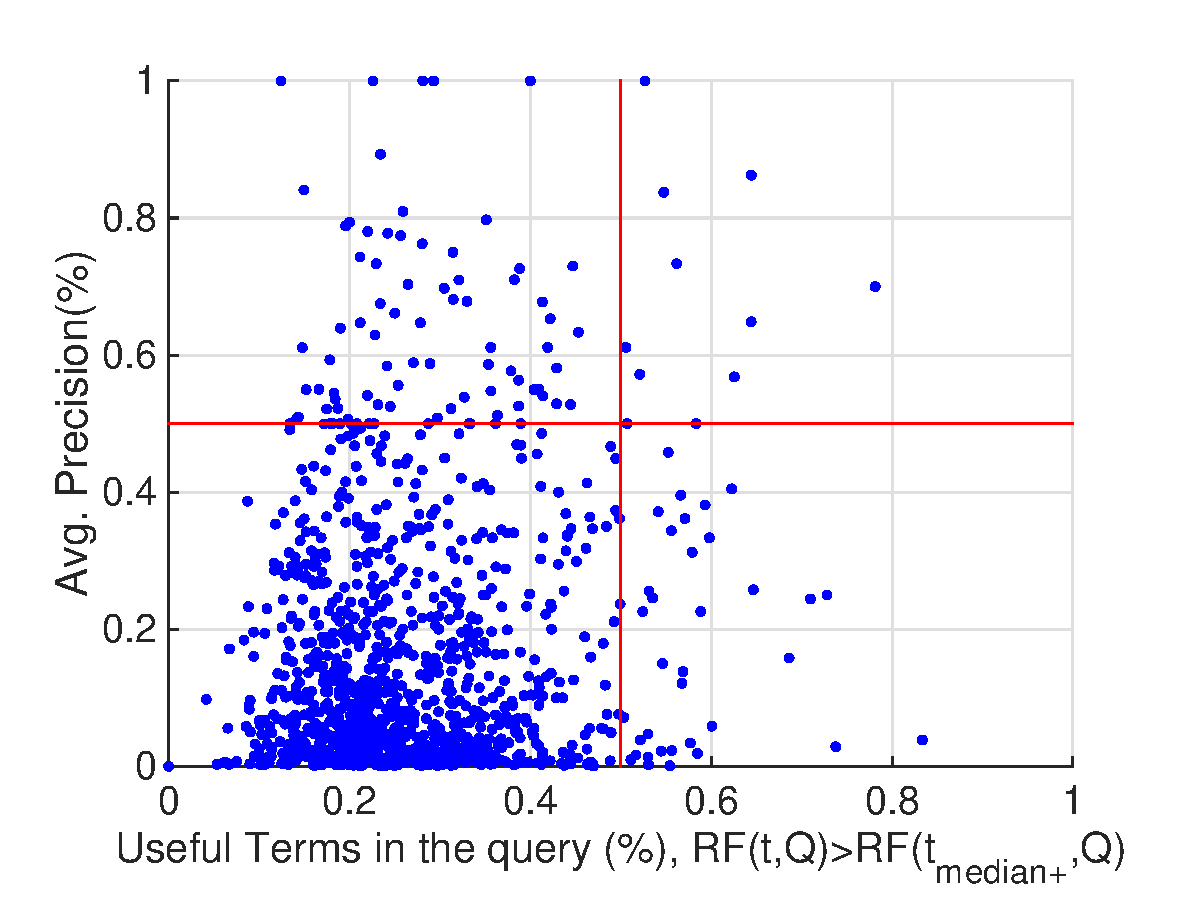
\includegraphics[width=5cm]{figs/greaterthammedian-p.eps}} \\%[-2ex]% 
\subfigure[{Useful terms: $ \{t|RF(t, Q)>1 \}$}]{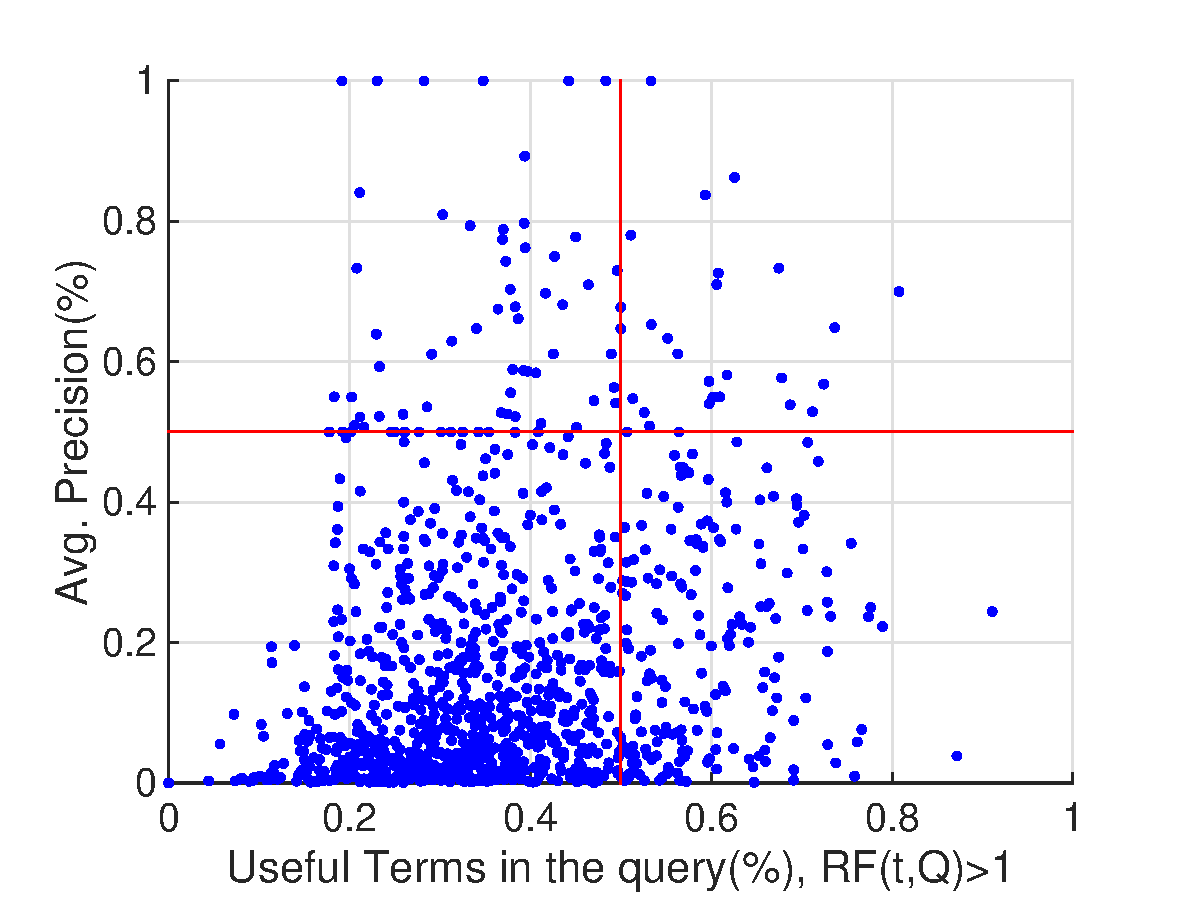
\includegraphics[width=5cm]{figs/greaterthan1-p.eps}} \hspace*{1.5cm} \subfigure[{Useful terms: top 100 high-scored terms}]{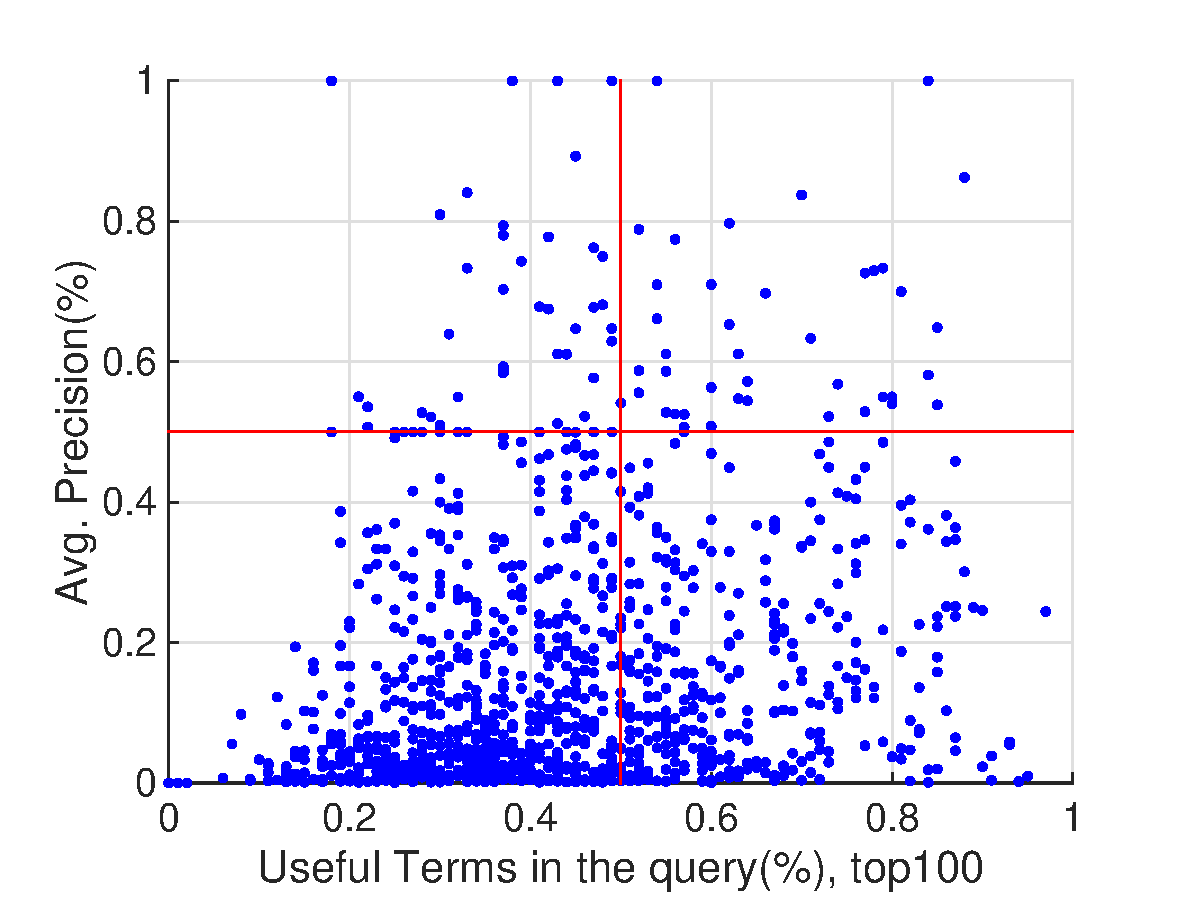
\includegraphics[width=5cm]{figs/top100-p.eps}}\\ %[-2ex]%
\subfigure[{Useful terms:$ \{t|score(t,Q)>5 \}$}]{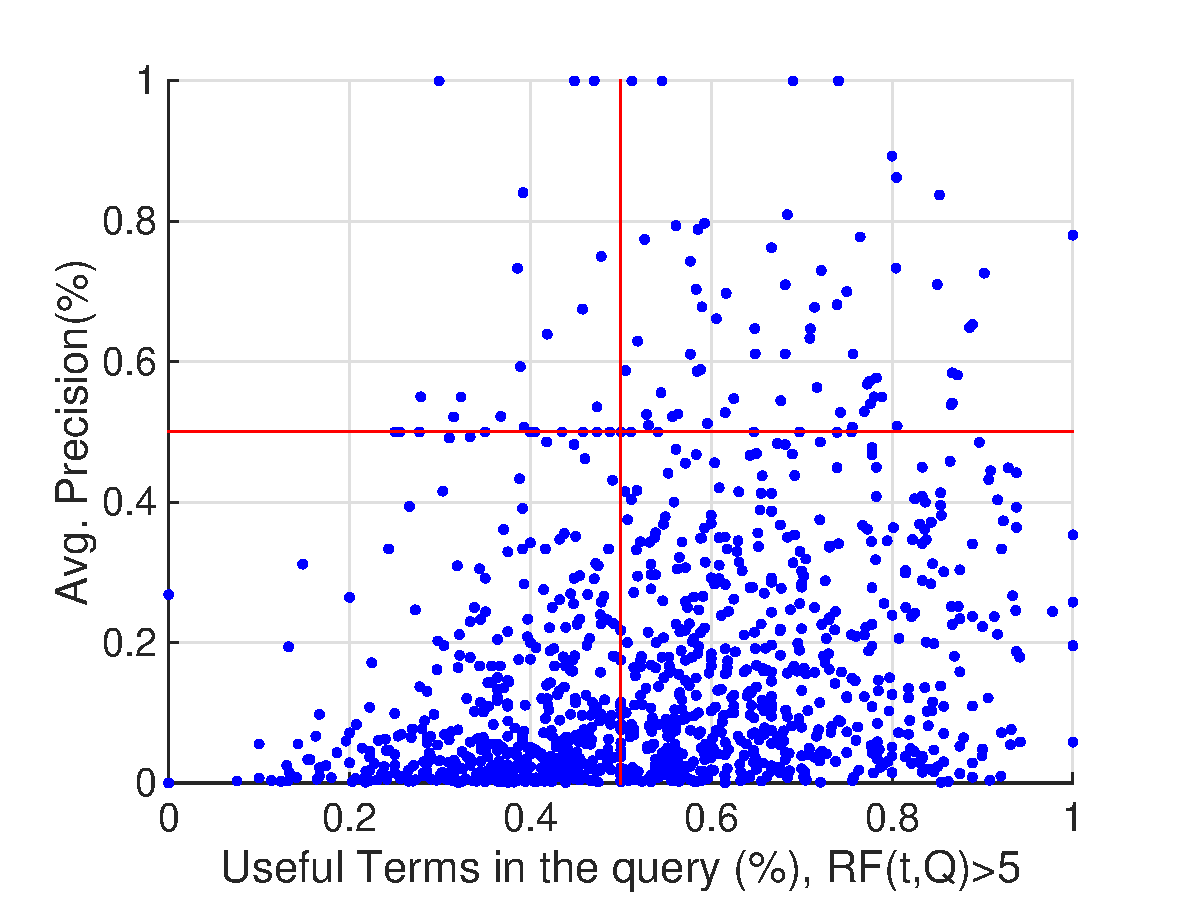
\includegraphics[width=5cm]{figs/greaterthan5-p.eps}} \hspace*{1.5cm} \subfigure[{Useful terms: $ \{t|RF(t, Q)>10\} $}]{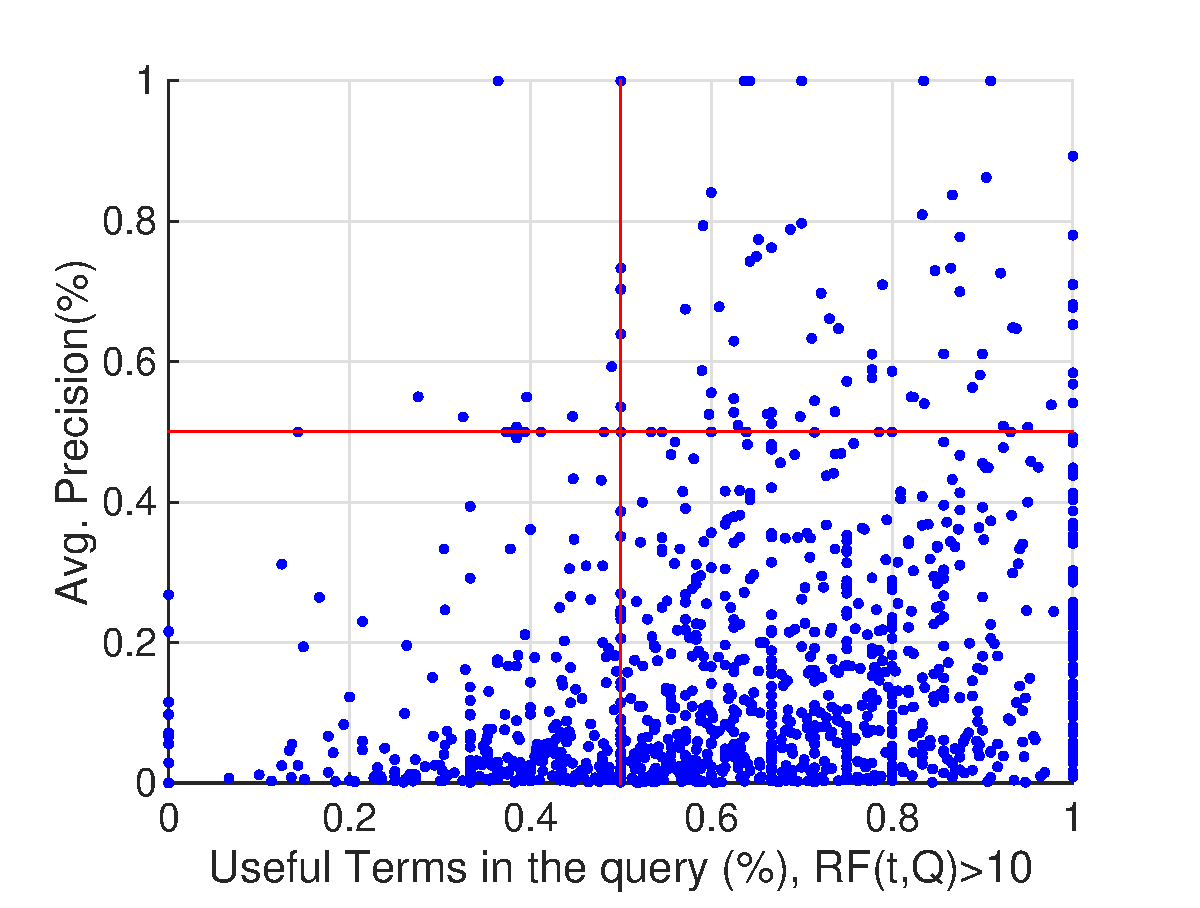
\includegraphics[width=5cm]{figs/greaterthan10-p.eps}}
\par\end{centering}

\protect\caption{Scatter plot of Average precision vs. the overlap between useful terms and the the query.}
\label{fig:overlap-p}
\end{figure}
%%%%%%%%%%%%%%%%%%%%%%%%%%%%%%%%%%%%%%%%%%%%%%%%%%%%%%%%%%%%%%
We expected to see a higher performance for the queries which contain more \textit{useful words} and a lower performance for the ones with less \textit{useful words}. However, unlike our first assumption, we could not find any correlation between the performance and the presence of \textit{useful words} in the query. The pattern for the recall is completely noisy while there is a very weak correlation between Average Precision and \textit{useful words} for top-scored words ($RF(t, Q)>10$). This experiment indicates that we should seek for reasons beyond the existence of the useful terms inside the query.  

Second, we check the term overlap with \textit{useful words} and \textit{noisy words} for TPs and FPs. Figure \ref{fig:usefulnoisy} shows that relevant patents have a higher term overlap with the \textit{useful words} while irrelevant patents have a higher term overlap with the \textit{noisy words}. This experiment shows that noisy words mislead the system to retrieve irrelevant patents at top of the list. 
%%%%%%%%%%%%%%%%%%%%%%%%%%%%%%%%%%%%%%%%%%%%%%%%%%%%%%%%%%%%%%
\begin{figure}[t!]
\begin{centering}
\subfigure[TPs]{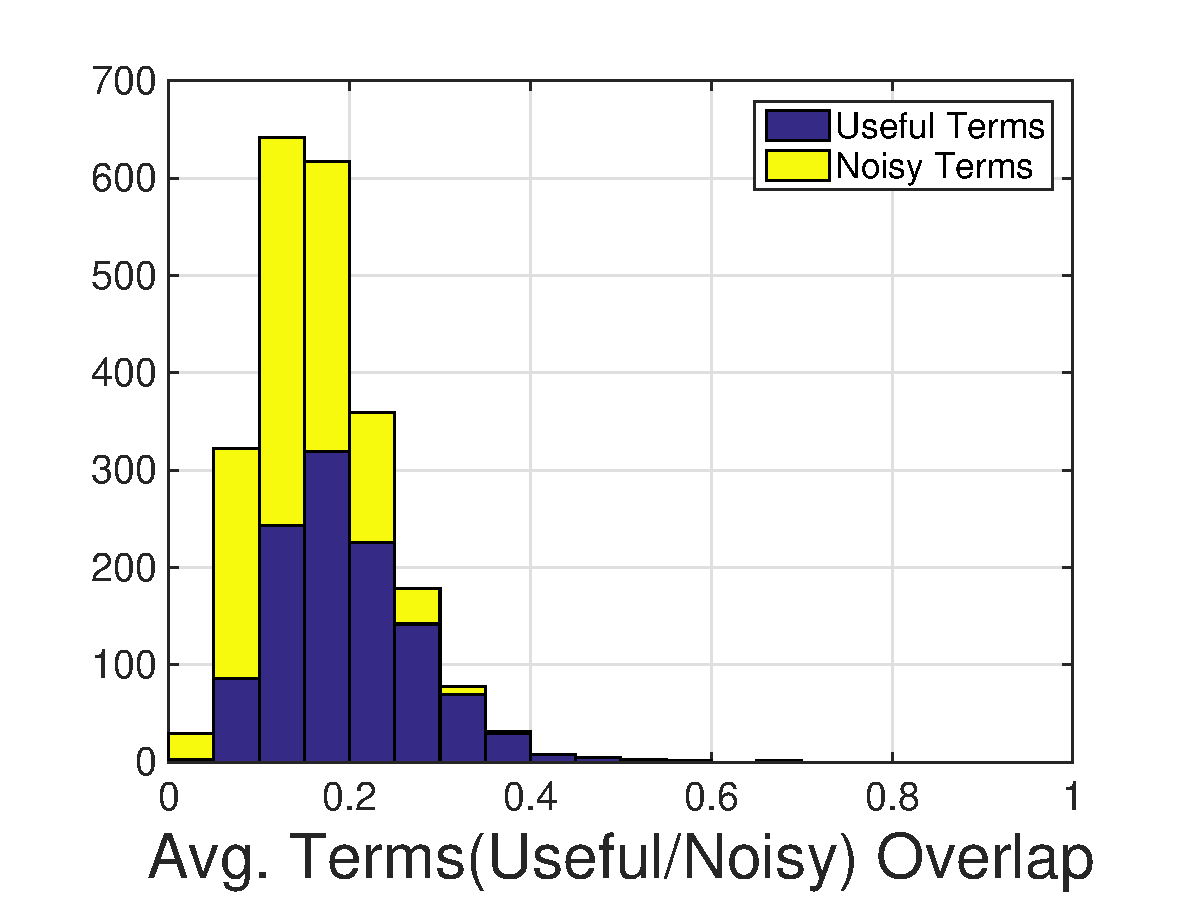
\includegraphics[width=6cm]{figs/stackedTPs.eps}} \hspace*{1.5cm} \subfigure[FPs]{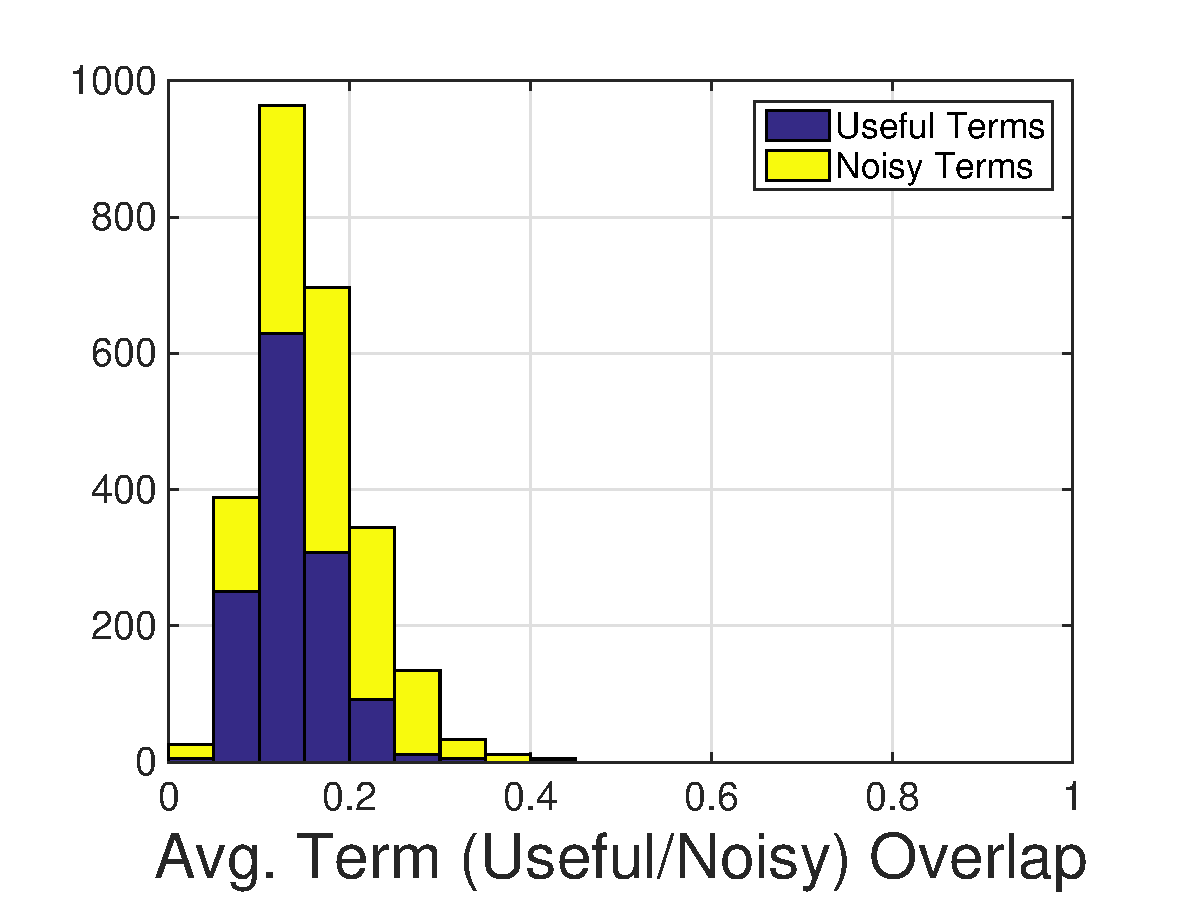
\includegraphics[width=6cm]{figs/stackedFPs.eps}} 
\par\end{centering} 

\protect\caption{The distribution of the term overlap between the query and useful words/noisy words in TPs and FPs.}
\label{fig:usefulnoisy}
\end{figure}
%%%%%%%%%%%%%%%%%%%%%%%%%%%%%%%%%%%%%%%%%%%%%%%%%%%%%%%%%%%%%%
%We hypothesized that a query, formulated by only the \textit{ useful terms}, is the best possible query we can make since they are all frequent in relevant patents but rare in irrelevant ones. 
\newpage
\subsection{Oracular Query Formulation}
\label{sec:OracularQueryFormulation}
In this section, we examine the system effectiveness for queries formulated using oracular Relevance Feedback ($\mathit{RF}$) system.

First, we formulate a query by selecting terms in the top-100 retrieved documents using oracular Relevance Feedback score and we call it oracular query. 
%%%%%%%%%%%%%%%%%%%%%%%%%%%%%%%%%%%%%%%%%%%%%%%%%%%%%%%%%%%%%%
\begin{equation}
Oracular \; Query = \{t \in top-100|RF(t, Q)>\tau\}   
 \label{eq:score}
\end{equation}
%%%%%%%%%%%%%%%%%%%%%%%%%%%%%%%%%%%%%%%%%%%%%%%%%%%%%%%%%%%%%% 
We empirically seek to evaluate the threshold $\tau$ on $RF(t,Q)$ and query size yielding the best oracular query.
%%%%%%%%%%%%%%%%%%%%%%%%%%%%%%%%%%%%%%%%%%%%%%%%%%%%%%%%%%%%%%
\begin{table}[t!]
  \begin{center}
  \scriptsize
   \caption{Performance for the \textit{Patent Query}, \textit{ Oracular Query}, and \textit{ Top CLEF-IP 2010 (PATATRAS)}.}
   \vspace*{1ex}
  \input table/optquery.tex   
  \label{tab:optquery}
  \end{center}  
\end{table}
%%%%%%%%%%%%%%%%%%%%%%%%%%%%%%%%%%%%%%%%%%%%%%%%%%%%%%%%%%%%%%
%%%%%%%%%%%%%%%%%%%%%%%%%%%%%%%%%%%%%%%%%%%%%%%%%%%%%%%%%%%%%%
\begin{figure}[t!]
\begin{centering}
\subfigure[Oracular query performance versus the threshold $\tau$.\label{fig:oracular-a}]{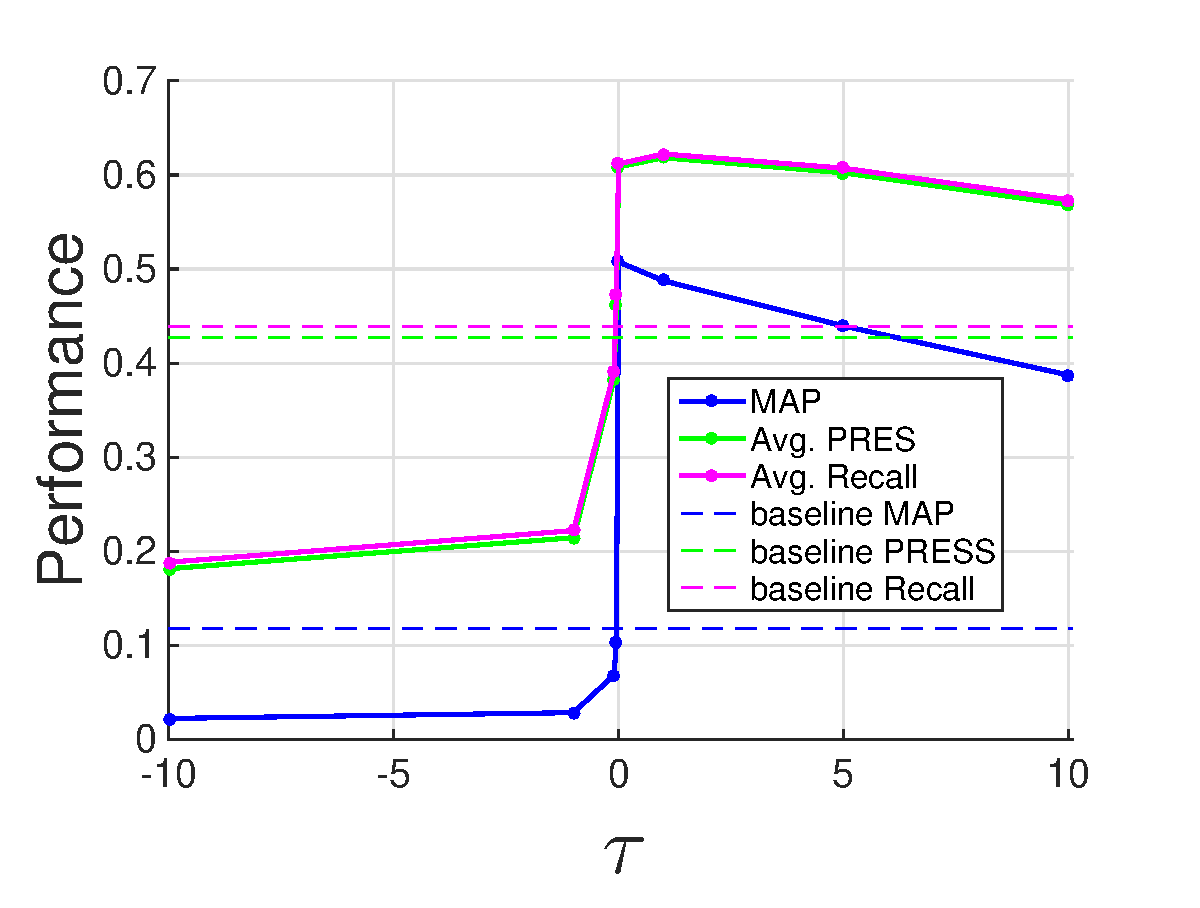
\includegraphics[width=6cm]{figs/oracularq.eps}} \hspace*{1.5cm} \subfigure[Oracular query performance versus the query size.\label{fig:oracular-b}]{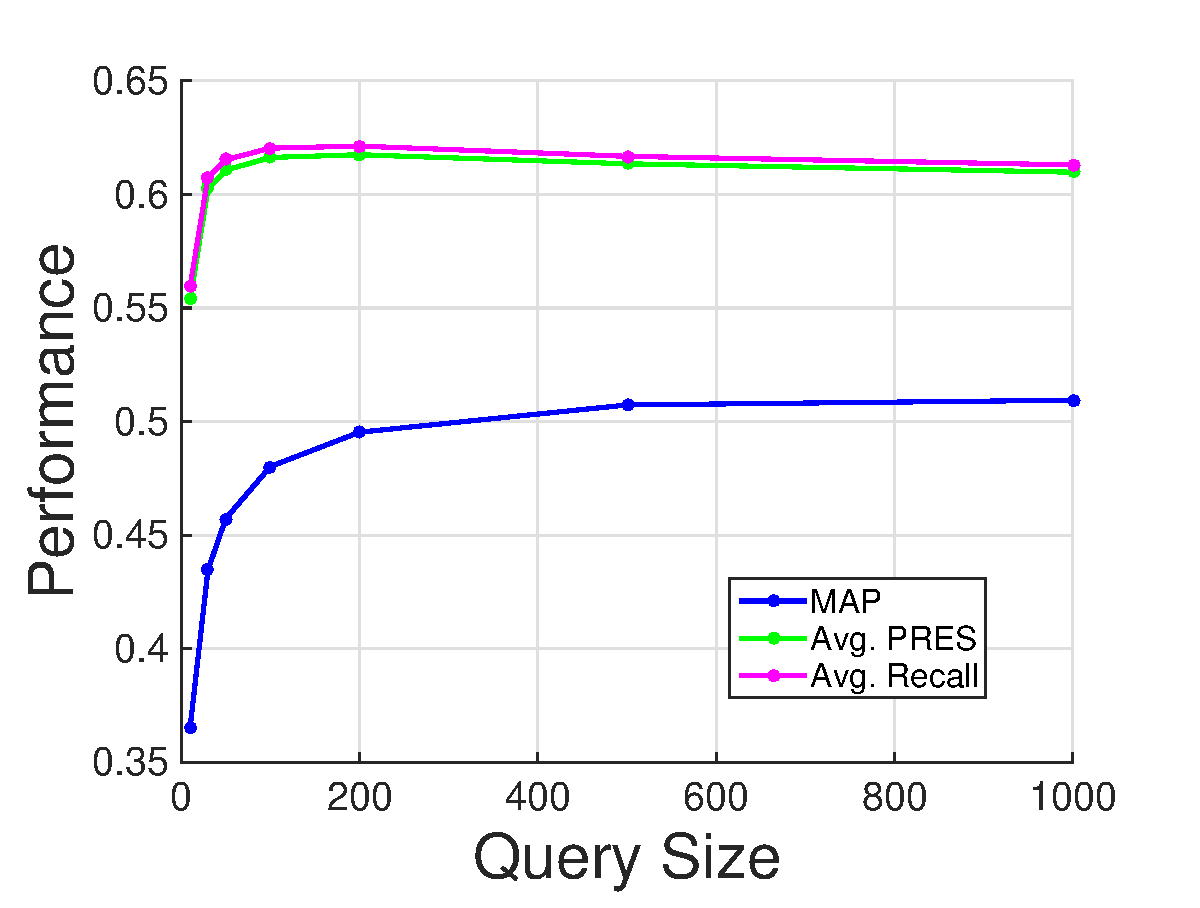
\includegraphics[width=6cm]{figs/oracularq-size.eps}} 
\par\end{centering} 
\protect\caption{Comparing the oracular query performance versus the threshold $\tau$ and query size}
\label{fig:oracular}
\end{figure}
%%%%%%%%%%%%%%%%%%%%%%%%%%%%%%%%%%%%%%%%%%%%%%%%%%%%%%%%%%%%%%

Figure \ref{fig:oracular} and Table \ref{tab:optquery} show that the oracular query far outperform the baseline, where the query is the reference patent query, and approximately performs twice as well on the PATATRAS system, the best competitor in CLEF-IP 2010 system. In Table \ref{tab:optquery}, we also compare the influence of weighed and unweighed terms for baseline and oracular query. It can be seen that weighing patent query terms with their frequency helps the performance while weighing oracular query terms with $RF(t, Q)$ harms the performance.  Figure \ref{fig:oracular-a} illustrates two main facts: First, the best-performed oracular query can be formulated by selecting the threshold $\tau=0$; Second, including slightly noisy terms (i.e., $\tau$ just slightly less than 0) gives rise to an unexpected steep drop-off in performance. Figure \ref{fig:oracular-b} shows that the performance increases notably when we include terms up to 200 while formulating a query, but it remains quit unchanged when we include more than 200 terms. 

Next, inspired by Maxwell and Croft's work~\citep{maxwell2013compact} that emphasise on the importance of query words, we formulate the second query by selecting oracular terms that also occur in the reference patent query as follows:
%%%%%%%%%%%%%%%%%%%%%%%%%%%%%%%%%%%%%%%%%%%%%%%%%%%%%%%%%%%%%%
\begin{equation}
 Oracular \; Patent \; Query = \{t\in Q|RF(t, Q)>\tau\}   
 \label{eq:score}
\end{equation}
%%%%%%%%%%%%%%%%%%%%%%%%%%%%%%%%%%%%%%%%%%%%%%%%%%%%%%%%%%%%%%
%%%%%%%%%%%%%%%%%%%%%%%%%%%%%%%%%%%%%%%%%%%%%%%%%%%%%%%%%%%%%%
\begin{figure}[t!]
   \centering
   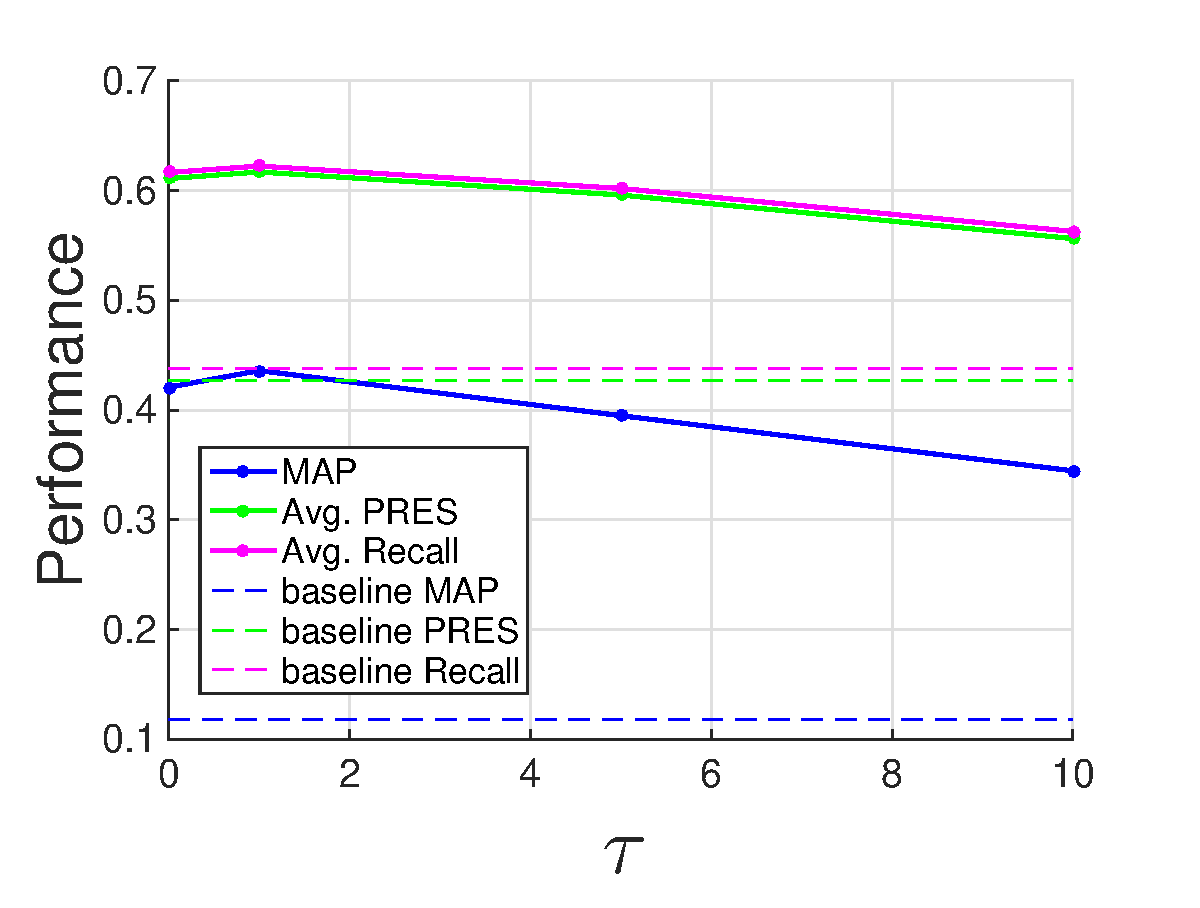
\includegraphics[width=0.50\textwidth,height=55mm]{figs/oracularpq.eps}
   \caption{oracular patent query performance versus the threshold $\tau$.}   
   \label{fig:oracularpq} 
\end{figure}
%%%%%%%%%%%%%%%%%%%%%%%%%%%%%%%%%%%%%%%%%%%%%%%%%%%%%%%%%%%%%%
The results for the Oracular Patent Query (Figure \ref{fig:oracularpq}) is also considerably improved compared to the baseline and PATATRAS again, though MAP is slightly less than Oracular Query. The results explain a very important fact that the patent query has sufficient terms for an improved performance and query expansion is not required in patent prior art search. We also conclude that the existence of the noisy words are the main cause of low effectiveness.  

Overall, our experiments related to oracular relevance feedback system
suggest two important conclusions: 
\begin{enumerate}
\item Query reduction should suffice for effective prior art patent retrieval; and 
\item Very precise methods for eliminating poor query terms in the reduction process are required.
\end{enumerate}

%\subsection{Discriminative Words}
%\label{sec:discriminative}
%
%\subsection{RF Optimal Query Formulation}
%\label{sec:formulation}

%%%%%%%%%%%%%%%%%%%%%%%%%%%%%%%%%%%%%%%%%%%%%%%%%%%%%%%%%%%%%%
%%%%%%%%%%%%%%%%%%%%%%%%% SECTION 3 %%%%%%%%%%%%%%%%%%%%%%%%%%
%%%%%%%%%%%%%%%%%%%%%%%%%%%%%%%%%%%%%%%%%%%%%%%%%%%%%%%%%%%%%%
\section{Query Reduction: Approximating the Oracular Patent Query}
The gain achieved using the Oracular Patent Query method motivates us to explore various methods to approximate the terms
selected by this query without ``peeking at the answers'' provided by
the actual relevance judgements.  We first attempt this via fully
automated methods and then proceed to evaluate semi-automated methods
based on interactive relevance feedback methods.
\subsection{Automated Reduction}
We use the following four simple features to reduce the initial patent queries and approximate the Oracular Patent Query: 
\begin{enumerate}
\item Document Frequent terms: In standard IR approaches, removing terms appearing highly frequently across documents in the collection can improve retrieval effectiveness~\citep{manning2008introduction}. Inspired by this fact, we assume that, after an initial run of the query, removing terms  with a high average document frequency (DF) over the top-100 documents improves the effectiveness. 
\item Frequent Terms in Query: Frequent terms inside long and verbose queries are considered important~\citep{maxwell2013compact}. Hence, we avoid removing frequent terms inside the query even if they are frequent in top-100 retrieved collection.
\item IPC Titles: The titles of classification indicate their intended content by using a single phrase or several related phrases linked together. We used words in IPC code titles for each patent query to reduce the query, based on the assumption that they are common to all patents belonging to the same category and may be considered as stop-words.
\item Pseudo Relevance Feedback ($\mathit{PRF}$): Pseudo relevance feedback is an automated process without user interaction which assumes the top k ranked documents are relevant and the others are irrelevant~\citep{Baeza-Yates2011}. We use $\mathit{PRF}$ to select query terms~\cite{maxwell2013compact} as we did with relevance feedback.
\end{enumerate}
We combine the first three features for our first query reduction approach. Pseudo relevance feedback is the second approach we yield to reduce the reference patent query. 
\subsubsection{Combined Approach}
First, we hypothesize that we will improve the performance by pruning out highly frequent words in top-100 retrieved documents from the patent query. For each word, we calculate the average term frequency over top-100 documents and call it Document Frequent (DF) score:
%%%%%%%%%%%%%%%%%%%%%%%%%%%%%%%%%%%%%%%%%%%%%%%%%%%%%%%%%%%%%%
\begin{equation}
 DF(t, Q)=\frac{1}{100}\sum_{d_i\in  D} TF(t, d_i)    
 \label{eq:df}
\end{equation}
where $D=\{d\in \mbox{Top-100 retrieved documents}\}$, and $TF(t, d_i)$ is the term frequency of each term in document $d_i$.
%\begin{displaymath}   t\in \lbrace \mbox{terms in top-100 retrieved documents}\rbrace\end{displaymath}
%%%%%%%%%%%%%%%%%%%%%%%%%%%%%%%%%%%%%%%%%%%%%%%%%%%%%%%%%%%%%%
%%%%%%%%%%%%%%%%%%%%%%%%%%%%%%%%%%%%%%%%%%%%%%%%%%%%%%%%%%%%%%
\begin{figure}[t!]
\begin{centering}
\subfigure[Mean Average Precision.]{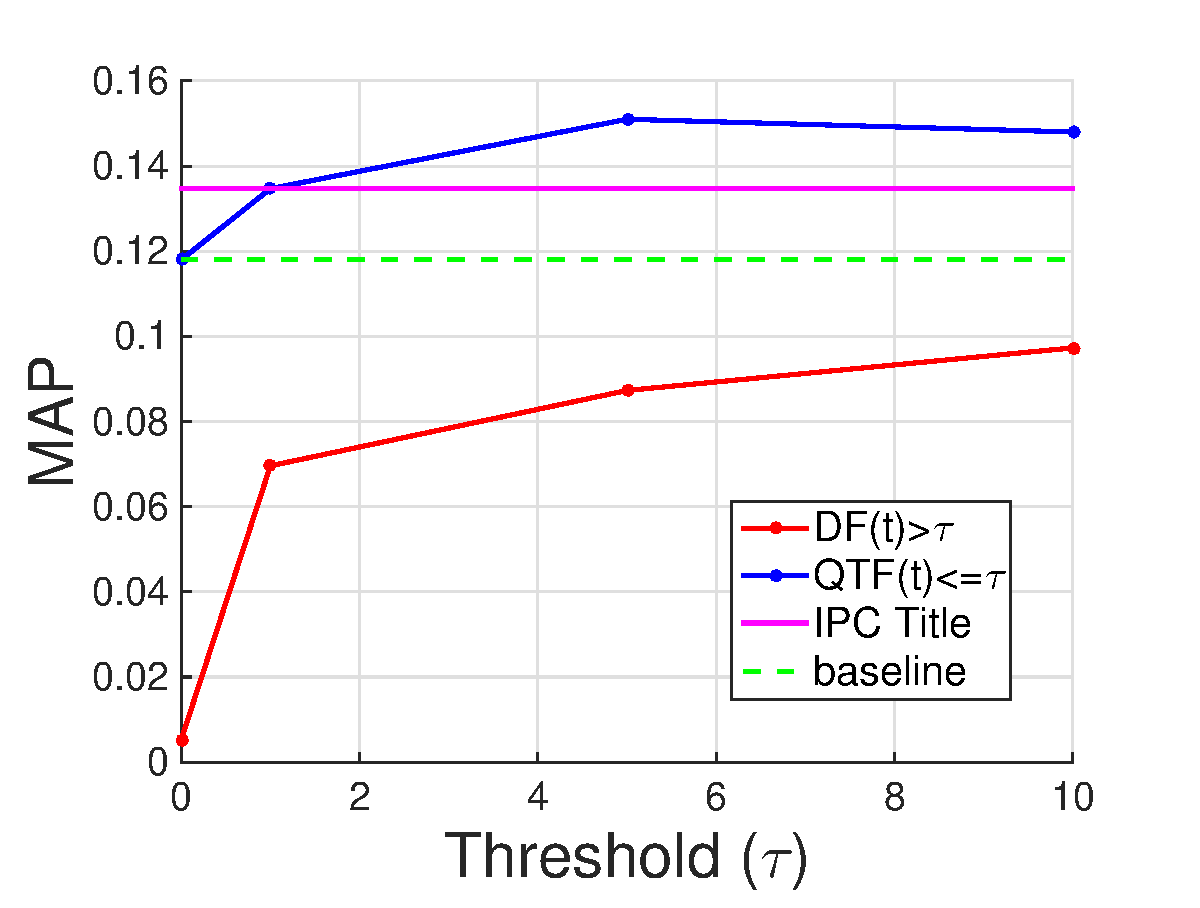
\includegraphics[width=6cm]{figs/combinedMAP.eps}} \hspace*{1.5cm} \subfigure[Average Recall.]{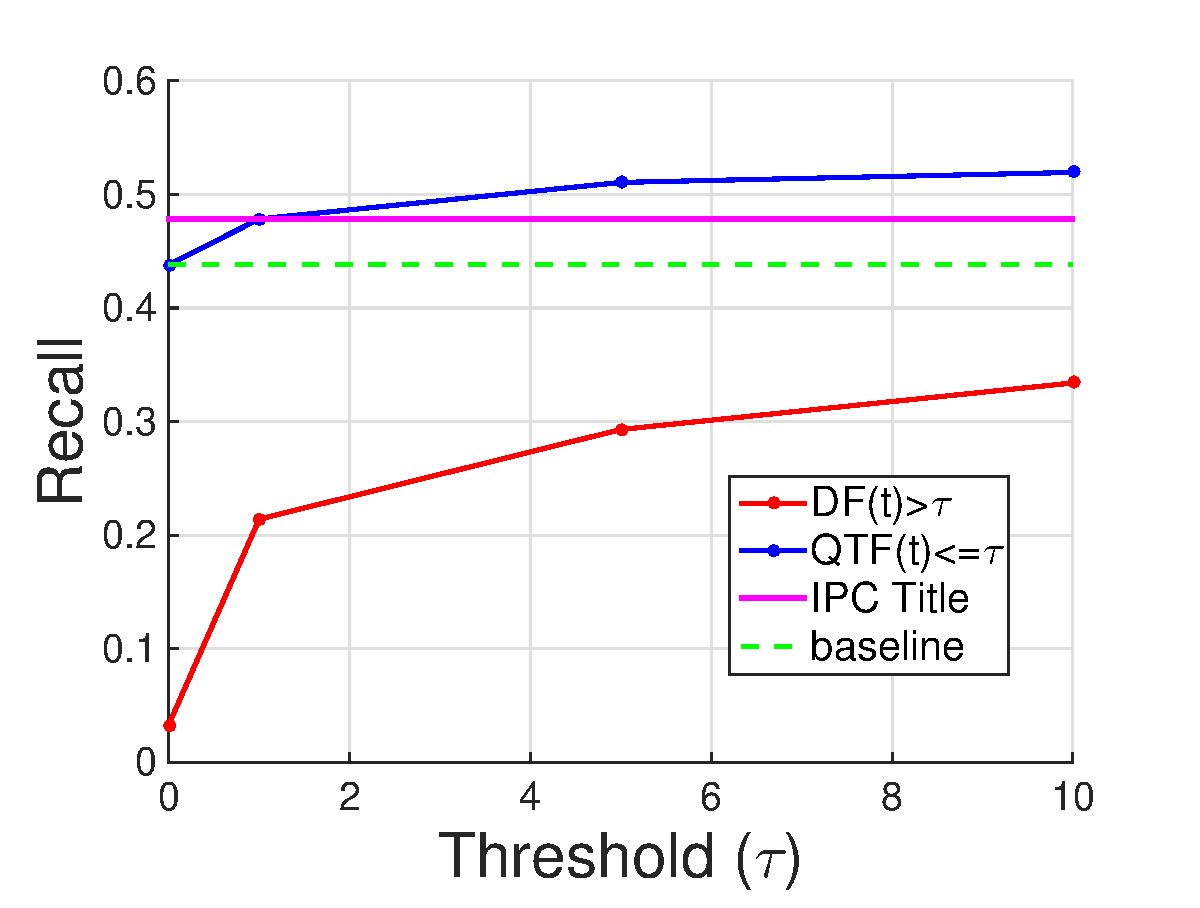
\includegraphics[width=6cm]{figs/combinedRecall.eps}} 
\par\end{centering} 
\protect\caption{System performance vs. the threshold for four query reduction approaches.}
\label{fig:combinedapproach}
\end{figure}
%%%%%%%%%%%%%%%%%%%%%%%%%%%%%%%%%%%%%%%%%%%%%%%%%%%%%%%%%%%%%%
Figure~\ref{fig:combinedapproach} illustrates how removing document frequent words for different threshold $\gamma$ can hurt the performance (red line). Hence, we combine this feature with the second feature--- query frequent terms to remove document frequent terms while to keep query frequent terms:
%%%%%%%%%%%%%%%%%%%%%%%%%%%%%%%%%%%%%%%%%%%%%%%%%%%%%%%%%%%%%%
\begin{displaymath}( DF(t, Q)>0.01 \; \wedge \; QTF(t)<=\alpha )\end{displaymath}
%%%%%%%%%%%%%%%%%%%%%%%%%%%%%%%%%%%%%%%%%%%%%%%%%%%%%%%%%%%%%%
As Figure \ref{fig:combinedapproach} shows, keeping query frequent terms helps the performance jumping slightly over the baseline. We empirically found out that $\gamma=0.01$ perform the best when we keep query frequent terms. The results also show that the best value for $\alpha$ is 5.

In the combined approach, we added the third feature --- IPC Title --- to also remove terms which are general in patents with the same IPC code: 
%%%%%%%%%%%%%%%%%%%%%%%%%%%%%%%%%%%%%%%%%%%%%%%%%%%%%%%%%%%%%%
\begin{displaymath} \left(  \left(DF(t, Q)>0.01\; \wedge \; QTF(t)<=5\right)\; \vee\; Query.contains(IPC \; Title \; words) \right)\end{displaymath}
%%%%%%%%%%%%%%%%%%%%%%%%%%%%%%%%%%%%%%%%%%%%%%%%%%%%%%%%%%%%%%
The results in Figure~\ref{fig:combinedapproach} (magenta line) show that removing IPC Title words from the reference patent query harms the performance. We did not assign any threshold for this feature we just removed document frequent words ($DF(t, Q)>0.01$) but we kept frequent words in the query ($QTF(t)>5$), then we removed words appeared in IPC Titles.   
%%%%%%%%%%%%%%%%%%%%%%%%%%%%%%%%%%%%%%%%%%%%%%%%%%%%%%%%%%%%%%
\begin{figure}[t!]
\begin{centering}
\subfigure[Query terms vs. Document Frequent terms.\label{fig:scatter_combined_a}]{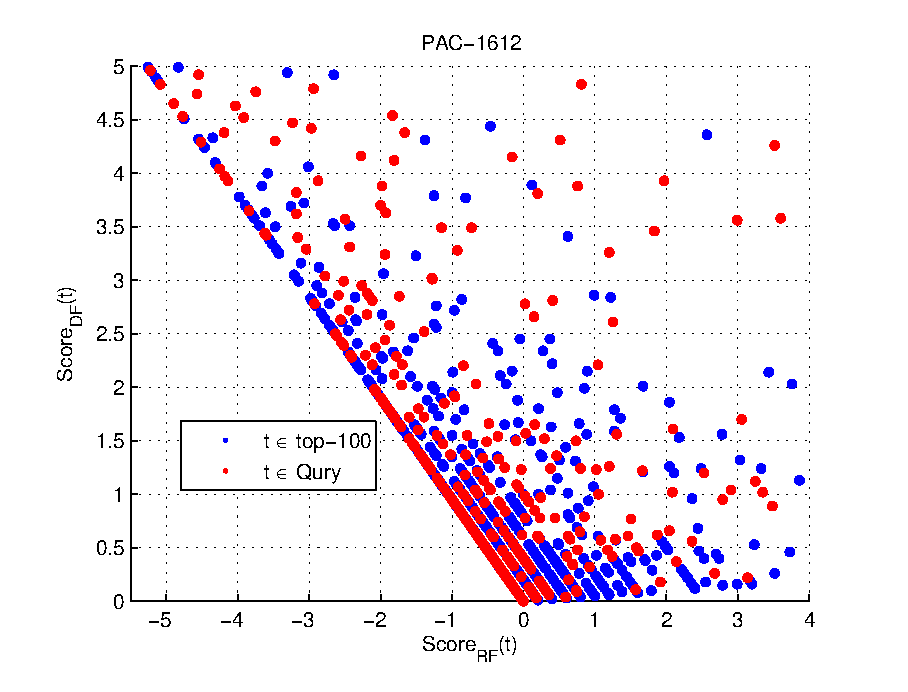
\includegraphics[width=9cm]{figs/qterm_rf_df.eps}} \hspace*{0.1cm}\\[1ex]% 
 %\subfigure[IPC Title words vs. Document Frequent terms.\label{fig:scatter_combined_b}]{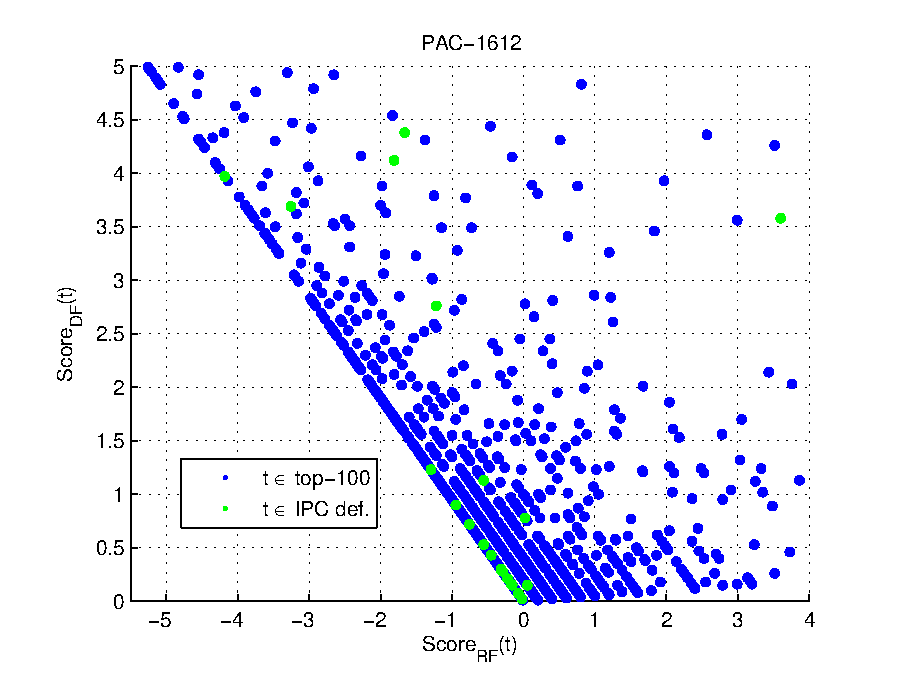
\includegraphics[width=7cm]{figs/ipcdef-rf-df.eps}} 
\subfigure[Remove document frequent terms while keeping query terms.\label{fig:scatter_combined_b}]{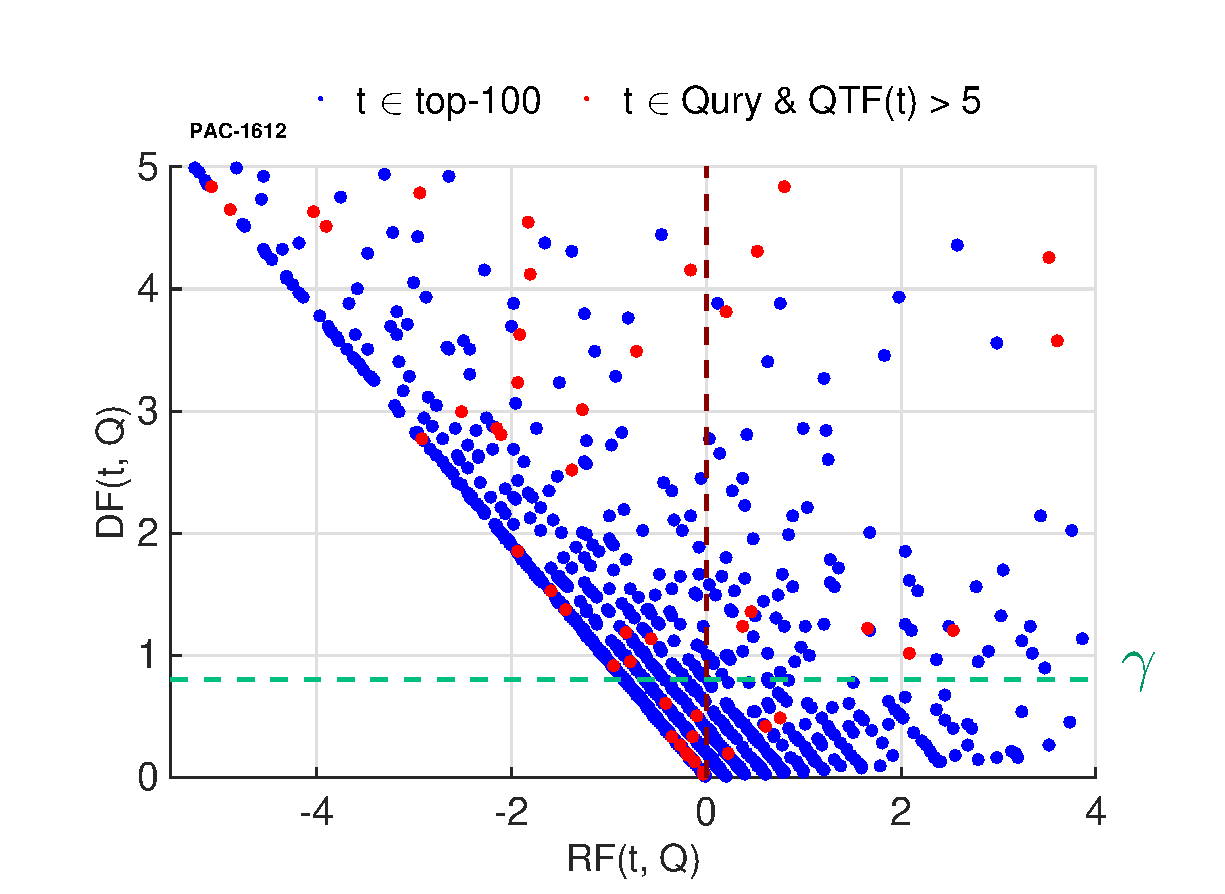
\includegraphics[width=9cm]{figs/df-rf-tauline.eps}}

\par\end{centering}

\protect\caption{Anecdotal example for combined approach.}
\label{fig:scatter_combined}
\end{figure}
%%%%%%%%%%%%%%%%%%%%%%%%%%%%%%%%%%%%%%%%%%%%%%%%%%%%%%%%%%%%%%

Figure~\ref{fig:scatter_combined_b} illustrates the combined approach. Each blue point is a vocabulary in top-100 retrieved document vocabulary set. First, we remark a negative correlation between $\mathit{DF(t, Q)}$ and $\mathit{RF(t, Q)}$, however, it does not help because as it can be seen we remove many useful terms ($RF(t, Q)>0$) by removing document frequent terms ($DF(t, Q)>\gamma$). Red points in Figure~\ref{fig:scatter_combined_b} are query terms with term frequency higher than 5, where we got the best performance in combined approach. We can see that we would avoid removing useful terms by keeping query frequent terms. Figure~\ref{fig:scatter_combined_a} shows that the sample patent query is contaminated by noisy words and Figure~\ref{fig:scatter_combined_b} shows that although the most of IPC Title words are noisy words, removing only few words that are useful can degrade the performance.    
\subsubsection{Pseudo Relevance Feedback}
% TODO: Must be consistent in either pruning or removing terms --- results should ideally converge to the baseline at 0.
% TODO: Should do simplest comparisons first and not combine pruning approaches.  Even better: evaluate methods mentioned in related work.
%\vspace*{0.5mm}
%\noindent \textbf{(1)} In standard IR approaches, removing terms appearing highly frequently across documents in the collection can improve retrieval effectiveness. Inspired by this fact, after an initial run of the query, we removed terms  with a high average document frequency (DF) over the top-100 documents ($\mathit{DF}(t)>\tau$). As illustrated in Figure \ref{fig:queryreduc}, such pruning significantly hurts performance.  
%
%\vspace*{0.5mm}
%\noindent \textbf{(2)} Frequent terms inside long and verbose queries have been shown to be important~\cite{maxwell2013compact}. Hence, we only keep high query TF (QTF) terms ($\mathit{QTF}(t)>\tau$) but remove from this set any document frequent terms ($\mathit{DF}(t)>0.01$).  Figure \ref{fig:queryreduc} indicates that this approach performs slightly better than the baseline.
%
%\vspace*{0.5mm}
%\noindent \textbf{(3)} The third query reduction approach is to select query terms using pseudo-relevance feedback ($\mathit{PRF}$)
%%~\cite{Baeza-Yates2011, maxwell2013compact}. 
%We calculated a $\mathit{PRF}$ score similar to $\mathit{RF}$ score assuming that the top-k ranked documents are relevant. We selected the query terms which have high $\mathit{PRF}$ score ($\mathit{PRF}(t)>\tau$). As Figure \ref{fig:queryreduc} illustrates, this approach does not notably outperform the baseline. 
%%In fact, we could not find any heuristic correlation between  $ PRF(t)$ and $ RF(t)$. 
%
%\vspace*{0.5mm}
%\noindent \textbf{(4)} Finally, we used words in IPC code title of each patent query to reduce the query, based on the assumption they are common to all patents, which belong to the same category and may be considered as stop-words. In our experiment, we removed the IPC title terms from a selection of frequent query terms ($QTF(t)>5$). We can see in Figure \ref{fig:queryreduc} that the results drop slightly compared to approach (2), where $\tau=5$.

% TODO: What is an IPC title?  I don't know that this is... was it discussed?
%%%%%%%%%%%%%%%%%%%%%%%%%%%%%%%%%%%%%%%%%%%%%%%%%%%%%%%%%%%%%%
\begin{figure}[t!]
   \centering
   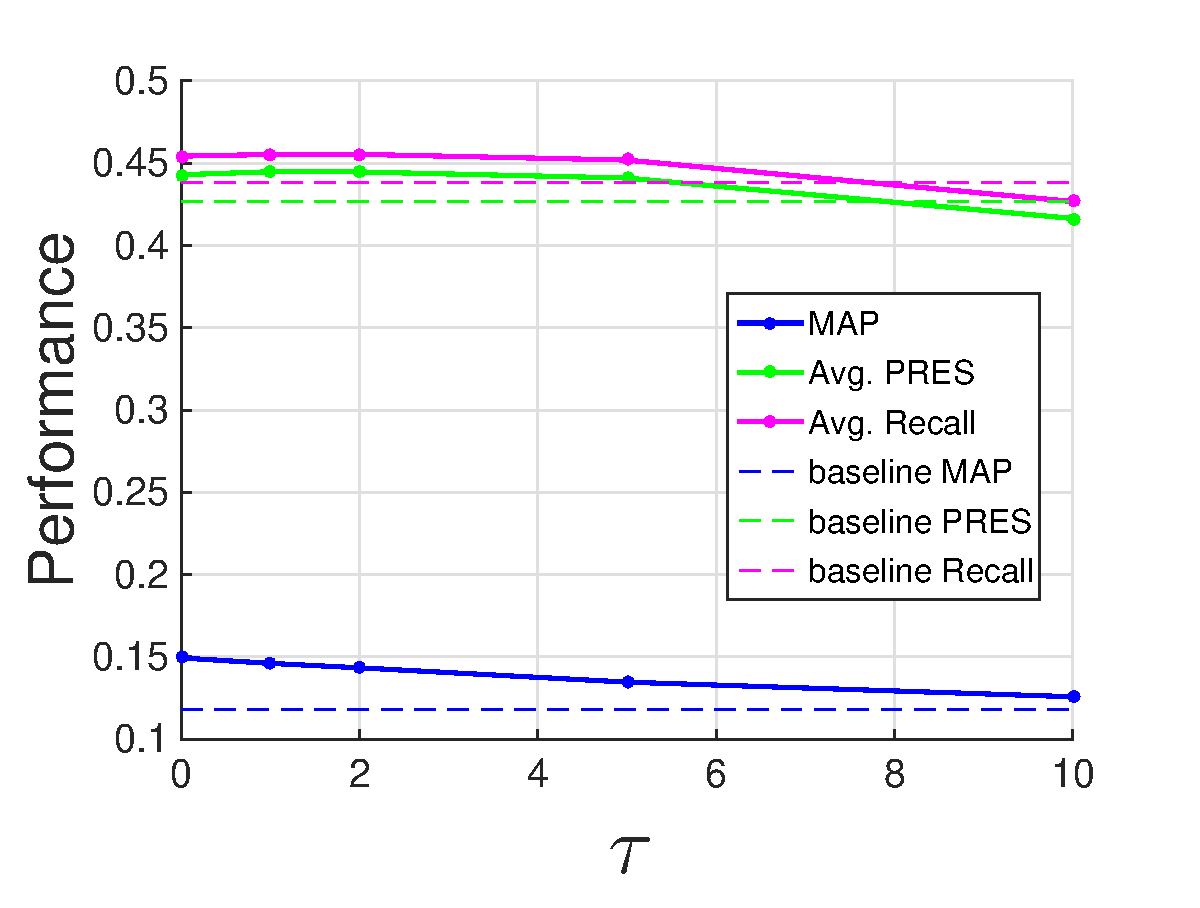
\includegraphics[width=0.50\textwidth,height=55mm]{figs/prf.eps}
   \caption{Query reduction using PRF for various value of the threshold $\tau$.}   
   \label{fig:prf} 
\end{figure}
%%%%%%%%%%%%%%%%%%%%%%%%%%%%%%%%%%%%%%%%%%%%%%%%%%%%%%%%%%%%%%
In this experiment, we use pseudo relevance feedback to select patent query terms, the same as what we did in oracular relevance feedback system (Section~\ref{sec:oraculrquery}). In pseudo relevance feedback, we assume that top 5 retrieved documents are relevant and the rest are irrelevant. We calculate pseudo relevance feedback score based on this assumption:  
%%%%%%%%%%%%%%%%%%%%%%%%%%%%%%%%%%%%%%%%%%%%%%%%%%%%%%%%%%%%%%
\begin{equation}
PRF(t,Q)=Rel(t)-Irr(t) 
 \label{eq:score}
\end{equation}
\vspace*{-2ex}
\begin{displaymath}t\in \lbrace \mbox{terms in top-100 retrieved documents}\rbrace\end{displaymath}
%%%%%%%%%%%%%%%%%%%%%%%%%%%%%%%%%%%%%%%%%%%%%%%%%%%%%%%%%%%%%%  
Then we just select the terms in patent query which have the pseudo relevance feedback score higher than threshold $\tau$ ($PRF(t)>\tau$) to formulate a reduced query. Figure~\ref{fig:prf} shows slight improvement over the baseline. However, the improvement is negligible compared to the oracular term selection system.
%%%%%%%%%%%%%%%%%%%%%%%%%%%%%%%%%%%%%%%%%%%%%%%%%%%%%%%%%%%%%%
\begin{figure}[t!]
\begin{centering}
\subfigure[$\tau=0$\label{fig:rf_prf_a}]{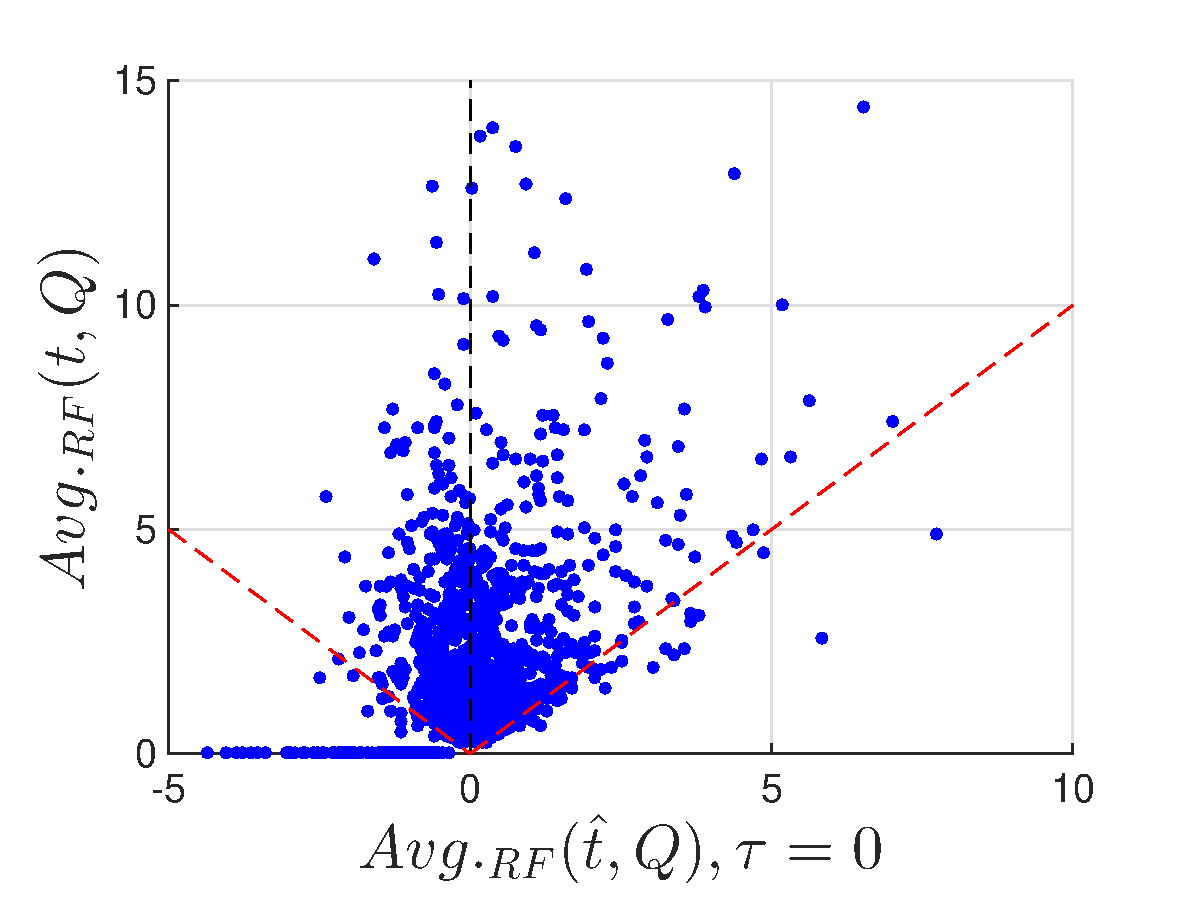
\includegraphics[width=7cm]{figs/scoretscorethat-tau0.eps}} \hspace*{0.1cm}
 \subfigure[$\tau=1$\label{fig:rf_prf_b}]{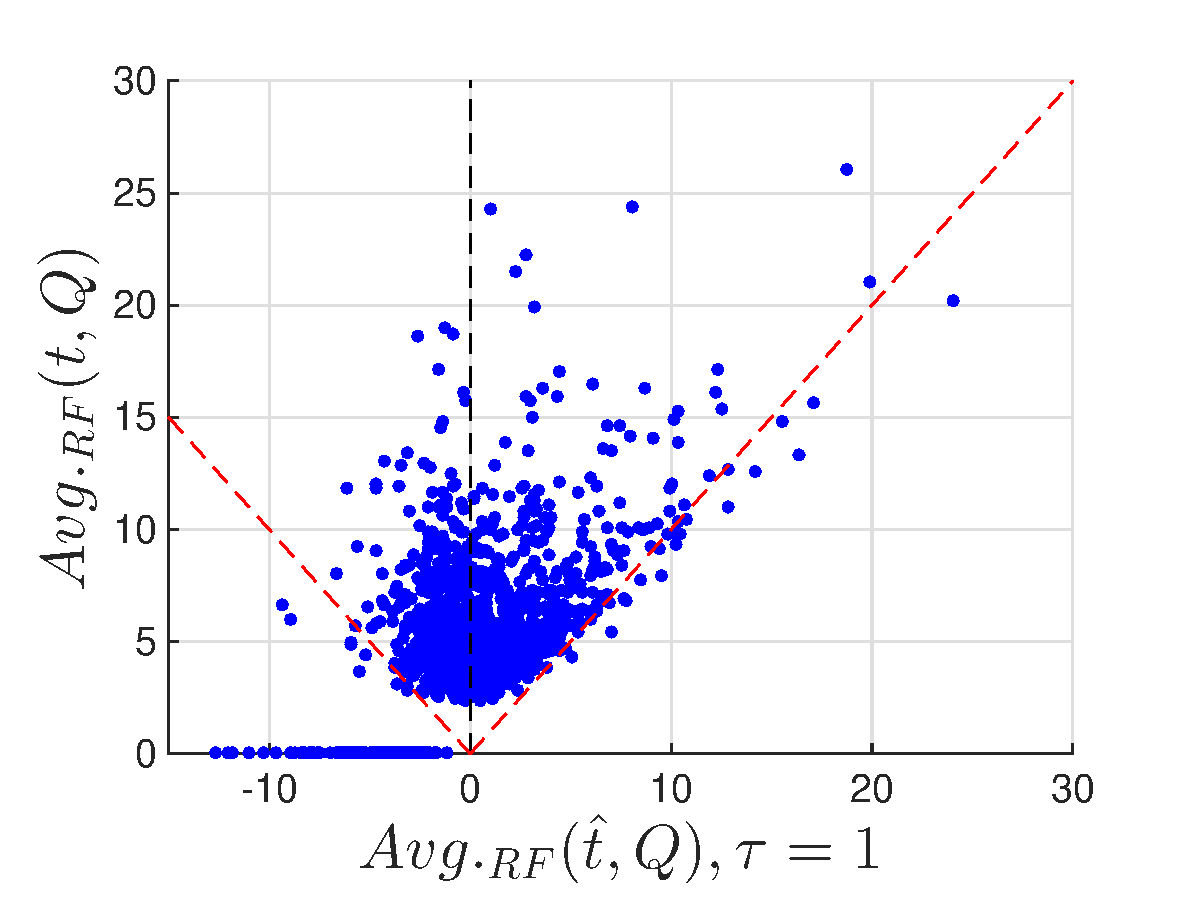
\includegraphics[width=7cm]{figs/scoretscorethat-tau1.eps}} \\[-1ex]% 
\subfigure[$\tau=10$\label{fig:rf_prf_c}]{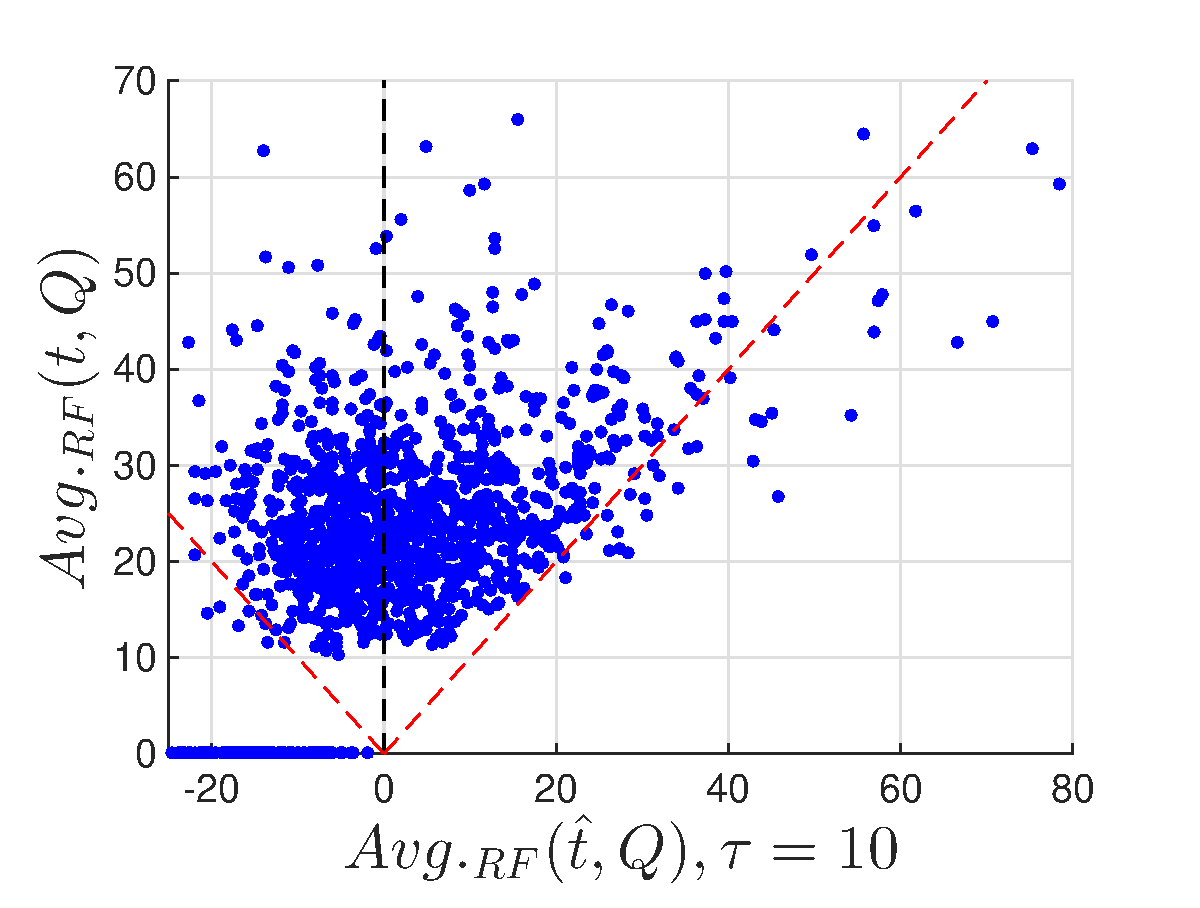
\includegraphics[width=7cm]{figs/scoretscorethat-tau10.eps}}

\par\end{centering}

\protect\caption{Comparing RF score of top relevance feedback terms and pseudo relevance feedback terms}
\label{fig:rf_prf}
\end{figure}
%%%%%%%%%%%%%%%%%%%%%%%%%%%%%%%%%%%%%%%%%%%%%%%%%%%%%%%%%%%%%%

In the following experiment, we seek for a pattern between top relevance feedback terms and top pseudo relevance feedback terms. We calculate the average RF score of both RF terms and PRF terms for each query as follows:
%%%%%%%%%%%%%%%%%%%%%%%%%%%%%%%%%%%%%%%%%%%%%%%%%%%%%%%%%%%%
\begin{equation}
Avg_{RF}(t, Q) = \frac{1}{|t|}\sum {RF}(t, Q), \;\;\;\; t\in \{t | RF(t, Q)>\tau\}
\end{equation}
%\begin{displaymath}t\in \{t | RF(t)>\tau\}\end{displaymath}
%%%%%%%%%%%%%%%%%%%%%%%%%%%%%%%%%%%%%%%%%%%%%%%%%%%%%%%%%%%%
\begin{equation}
Avg_{RF}(\hat{t}, Q) = \frac{1}{|\hat{t}|}\sum {RF}(\hat{t}, Q), \;\;\;\; \hat{t}\in \{\hat{t} | PRF(\hat{t}, Q)>\tau\} 
\end{equation}
%\begin{displaymath}\hat{t}\in \{\hat{t} | PRF(\hat{t})>\tau\}\end{displaymath}
%%%%%%%%%%%%%%%%%%%%%%%%%%%%%%%%%%%%%%%%%%%%%%%%%%%%%%%%%%%%
Figure~\ref{fig:rf_prf} justifies why pseudo relevance feedback is not as effective as relevance feedback. As it can be seen top pseudo relevance feedback terms consider noisy words based on their RF scores. Since there is no heuristics that correlates with relevance feedback and pseudo relevance feedback, we can not approximate the oracular query via pseudo relevance feedback.   
%%%%%%%%%%%%%%%%%%%%%%%%%%%%%%%%%%%%%%%%%%%%%%%%%%%%%%%%%%%%
\begin{figure}[htpb]
\begin{framed}
\vspace*{-2ex}
  \centering
    %\lstinputlisting[frame=single, basicstyle=\scriptsize\ttfamily , linewidth=\columnwidth,breaklines=true]{code/anecdotale.tex}\vspace*{-2ex}
 \begin{lstlisting}[basicstyle=\small\ttfamily , linewidth=\columnwidth,breaklines=true, language=TeX] 
PAC-1293

Abstract: The invention relates to an emulsifier, a method for 
preparing said emulsifier, and to its use in various applications
, primarily food and cosmetic applications. The invention also 
relates to the use of said emulsifier for the creation of an 
elastic, gelled foam. An emulsifier according to the invention is 
based on a starch which is enzymatically converted, using a 
specific type of enzyme, and modified in a specific 
esterification reaction.

DF Terms: <@\textcolor{blue}{starch:14.64}@>, <@\textcolor{blue}{enzym:29.49}@>, <@\textcolor{red}{amylos:-20.15}@>, 
<@\textcolor{blue}{oil:8.63}@>, <@\textcolor{red}{dispers:-8.66}@>, <@\textcolor{red}{ph:-4.55}@>, <@\textcolor{red}{dry:-6.21}@>, <@\textcolor{red}{heat:-2.26}@>, 
<@\textcolor{red}{product:-5.48}@>, <@\textcolor{red}{slurri:-11.48}@>, <@\textcolor{blue}{viscos:7.77}@>, <@\textcolor{red}{composit:-4.49}@>, 
<@\textcolor{red}{reaction:-1.97}@>, <@\textcolor{red}{food:-11.94}@>, <@\textcolor{blue}{agent:5.19}@>, <@\textcolor{red}{debranch:-10.58}@>, 
<@\textcolor{red}{reduc:-6.37}@>, <@\textcolor{red}{fat:-12.83}@>, <@\textcolor{red}{prepar:-0.82}@>, <@\textcolor{red}{hour:-5.42}@>, 
<@\textcolor{blue}{waxi:19.41}@>, <@\textcolor{blue}{deriv:11.97}@>, <@\textcolor{red}{content:-3.38}@>, <@\textcolor{blue}{aqueou:0.38}@>, 
<@\textcolor{red}{saccharid:-11.95}@>, <@\textcolor{red}{ml:-0.79}@>, <@\textcolor{red}{cook:-10.04}@>, <@\textcolor{blue}{modifi:5.65}@>, 
<@\textcolor{blue}{solid:5.50}@>, <@\textcolor{blue}{sampl:6.27}@>, <@\textcolor{blue}{mix:2.48}@>, <@\textcolor{red}{minut:-1.68}@>, <@\textcolor{red}{dri:-0.91}@>, 
<@\textcolor{red}{gel:-9.85}@>, <@\textcolor{blue}{activ:5.98}@>, <@\textcolor{red}{corn:-5.27}@>, <@\textcolor{blue}{alpha:12}@>, <@\textcolor{red}{sprai:-2.74}@> 

QTF Terms: <@\textcolor{blue}{starch:14.64}@>, <@\textcolor{blue}{emulsifi:6.72}@>, <@\textcolor{red}{succin:-3.46}@>, 
<@\textcolor{blue}{enzym:29.49}@>, <@\textcolor{blue}{emuls:12.66}@>, <@\textcolor{blue}{hydrophob:5.45}@>, <@\textcolor{red}{anhydrid:-5.47}@>, 
<@\textcolor{red}{reaction:-1.97}@>, <@\textcolor{red}{octenyl:-0.66}@>, <@\textcolor{blue}{stabil:3.64}@>, <@\textcolor{blue}{alkenyl:0.06}@>, 
<@\textcolor{blue}{reagent:1.17}@>, <@\textcolor{blue}{carbon:0.12}@>, <@\textcolor{blue}{potato:3.74}@>, <@\textcolor{red}{alkyl:-0.33}@>, 
<@\textcolor{red}{wt:-4.57}@>, <@\textcolor{blue}{ether:1.96}@>, <@\textcolor{red}{enzymat:-3.45}@>, <@\textcolor{blue}{convers:10.44}@>, 
<@\textcolor{red}{chain:-5.53}@>, <@\textcolor{blue}{atom:0.03}@>, <@\textcolor{red}{ph:-4.55}@>, <@\textcolor{red}{treat:-0.89}@>, 
<@\textcolor{red}{ammonium:-1.96}@>, <@\textcolor{red}{food:-11.94}@>, <@\textcolor{red}{amylos:-20.15}@>, 
<@\textcolor{red}{glucanotransferas:-0.86}@>, <@\textcolor{red}{glycidyl:-0.40}@>, <@\textcolor{red}{glycosyl:-0.02}@>, 
<@\textcolor{red}{dry:-6.21}@>, <@\textcolor{blue}{deriv:11.97}@>, <@\textcolor{blue}{transferas:0.89}@>, <@\textcolor{red}{foam:-0.49}@>, 

PRF Terms: <@\textcolor{blue}{starch:14.64}@>, <@\textcolor{blue}{encapsul:17.50}@>, <@\textcolor{red}{chees:-4.22}@>, 
<@\textcolor{blue}{oil:8.63}@>, <@\textcolor{blue}{hydrophob:5.45}@>, <@\textcolor{blue}{agent:5.19}@>, <@\textcolor{red}{casein:-2.19}@>, 
<@\textcolor{blue}{degrad:17.13}@>, <@\textcolor{blue}{deriv:11.97}@>, <@\textcolor{blue}{tablet:5.30}@>, <@\textcolor{red}{debranch:-10.58}@>, 
<@\textcolor{red}{imit:-1.13}@>, <@\textcolor{blue}{viscos:7.77}@>, <@\textcolor{blue}{oxid:5.97}@>, <@\textcolor{blue}{activ:5.98}@>, <@\textcolor{blue}{osa:9.32}@>, 
<@\textcolor{blue}{funnel:2.68}@>, <@\textcolor{blue}{amylas:26.06}@>, <@\textcolor{red}{amylopectin:-7.14}@>, <@\textcolor{blue}{maiz:20.61}@>, 
<@\textcolor{red}{blend:-3.17}@>, <@\textcolor{blue}{waxi:19.41}@>, <@\textcolor{blue}{convert:31.81}@>, 

IPC title Terms:<@\textcolor{blue}{cosmet:3.77}@>, <@\textcolor{blue}{toilet:0.18}@>, <@\textcolor{red}{prepar:-0.82}@>, 
<@\textcolor{blue}{case:0.47}@>, <@\textcolor{red}{accessori:-0.01}@>, <@\textcolor{red}{store:-0.37}@>, <@\textcolor{blue}{handl:0.07}@>, 
<@\textcolor{red}{pasti:-0.17}@>, <@\textcolor{red}{substanc:-1.21}@>, <@\textcolor{red}{fibrou:-0.01}@>, <@\textcolor{red}{pulp:-1.28}@>, 
<@\textcolor{red}{constitut:-0.06}@>, <@\textcolor{blue}{paper:1.26}@>, <@\textcolor{red}{impregn:-0.11}@>, <@\textcolor{blue}{emulsifi:6.72}@>, 
<@\textcolor{red}{wet:-0.28}@>, <@\textcolor{red}{dispers:-8.66}@>, <@\textcolor{red}{foam:-0.49}@>, <@\textcolor{red}{produc:-0.57}@>, 
<@\textcolor{blue}{agent:5.19}@>, <@\textcolor{blue}{relev:0.18}@>, <@\textcolor{blue}{class:0.053}@>, <@\textcolor{red}{lubric:-0.38}@>, 
<@\textcolor{blue}{emuls:12.66}@>, <@\textcolor{red}{fuel:-0.011}@>, <@\textcolor{blue}{deriv:11.97}@>, <@\textcolor{blue}{starch:14.64}@>, 
<@\textcolor{red}{amylos:-20.15}@>, <@\textcolor{red}{compound:-0.63}@>, <@\textcolor{red}{saccharid:-11.95}@>, 
<@\textcolor{blue}{radic:1.03}@>, <@\textcolor{red}{acid:-3.19}@> 
 \end{lstlisting} 
 \vspace*{-2ex}
\end{framed}
 \vspace*{-2ex}
  \caption{Four query reduction approaches on a sample query.  Top
    terms retained by each method are shown.  Numerical oracular
    scores $\mathit{RF}(t,Q)$ are provided indicating whether the term
    was useful (blue/positive) or noisy (red/negative).}
  \label{fig:anecdotal}  
\end{figure}
%\FloatBarrier
%%%%%%%%%%%%%%%%%%%%%%%%%%%%%%%%%%%%%%%%%%%%%%%%%%%%%%%%%%%%

We justify the reason that four mentioned query reduction approaches could not compete with our oracular query via following anecdotal example. 
Figure \ref{fig:anecdotal} shows an anecdotal example for a sample query about an invention related to ``emulsifier'' to help explain why these four approaches fail. It shows the raw abstract of the invention, and terms and their associated $\mathit{RF}$ scores for each approach. In Figure \ref{fig:anecdotal} terms are chosen for each approach  as follows: 
\begin{displaymath}\{t| DF(t)/QTF(t)/PRF(t)>10\}\end{displaymath}
%$\{t| DF(t)/QTF(t)/PRF(t)>10\}$.
IPC title terms are the words appearing in the IPC title and do not have any score.

It can be seen that the four methods fail clearly to discriminate between useful and noisy terms. As one example, important stemmed terms like ``enzym'' and ``starch'' have been removed by DF pruning in (1), which hurts query quality.  As another example, retaining IPC code title terms yields more noisy terms than useful terms (19 out of 32, and few of them with a very negative score like ``amylos'' or ``saccharid''). Overall, while some methods like PRF work better than others for query reduction, all methods may retain highly negative terms and results from Section~\ref{sec:OracularQueryFormulation} showed that the inclusion of even slightly negative terms can significantly hurt performance.
\subsection{Semi-automated Interactive Reduction}
\label{sec:SemiAutomatedInteractiveReduction}

Our sample analysis of specific queries and terms selected via our oracular
approach suggests that automated methods fall far short of optimal term selection.
This leads us to explore another approach of approximating the oracular query
derived from relevance judgements by using a subset of relevance judgements
through interactive methods.  Specifically, to minimize the need for user interaction,
in this section we analyse the performance of an oracular query derived from
only the first relevant document identified in the search results.
%\begin{comment}
%All our attempts to improve the system effectiveness without accessing the relevance feedback were quite in vein because the features we recognized were tightly the combination of the useful words and noisy words and the system performance is too sensitive to the existence of a noisy word or the absence of the useful terms. So, we decided to apply much more realistic approach in which feedback terms are extracted only from the first ranked relevant document retrieved. 
%\end{comment}
Using this approach, Table \ref{tab:firstrel} shows that we can double the MAP in comparison to our baseline and also outperform the PATATRAS system.

%%%%%%%%%%%%%%%%%%%%%%%%%%%%%%%%%%%%%%%%%%%%%%%%%%%%%%%%%%%%%%%%
\begin{table}[t!]
  \begin{center}
   \caption{System performance using minimal relevance feedback. $\tau$ is RF score threshold, and $k$ indicates the number of first relevant retrieved patents.}\vspace{3mm}
  \input table/partialRFtermselect1.tex   
  \label{tab:firstrel}
  \end{center}  
\end{table}
%%%%%%%%%%%%%%%%%%%%%%%%%%%%%%%%%%%%%%%%%%%%%%%%%%%%%%%%%%%%%%%%

Furthermore, to establish the minimal interaction required by this
approach, Figure \ref{fig:FirstTPRankHisto} indicates that the
baseline methods return a relevant patent approximately 80\% of the
time in the first 10 results and 90\% of the time in the first 20
results.  Hence, such an interactive approach requires relatively low
user effort while achieving state-of-the-art performance.

%%%%%%%%%%%%%%%%%%%%%%%%%%%%%%%%%%%%%%%%%%%%%%%%%%%%%%%%%%%%%%%%
\begin{figure}
\begin{centering}
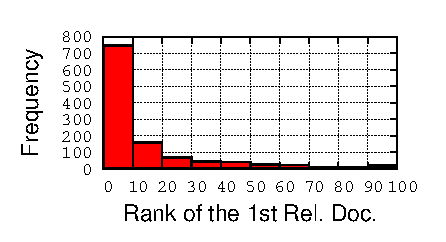
\includegraphics[width=6.5cm, height=3.5cm]{figs/1stRank}
\par\end{centering}

\protect\caption{The distribution of the first relevant document rank over test queries.}
\label{fig:FirstTPRankHisto}
\end{figure}
%%%%%%%%%%%%%%%%%%%%%%%%%%%%%%%%%%%%%%%%%%%%%%%%%%%%%%%%%%%%%%%%
%%%%%%%%%%%%%%%%%%%%%%%%% SECTION 4 %%%%%%%%%%%%%%%%%%%%%%%%%%
%%%%%%%%%%%%%%%%%%%%%%%%%%%%%%%%%%%%%%%%%%%%%%%%%%%%%%%%%%%%%%
\section{Section-based Analysis}
\textcolor{red}{Mona: I am not sure if this suits in this chapter, no idea where I can put them!}\\
Patents are structured documents containing Title, Abstract, Description, and Claims. In these series of experiments, we concentrate on sections to find out average number of useful terms in each section of the patent query. We also show which section is more useful in both Relevance Feedback and Pseudo Relevance Feedback.
%\subsubsection{Useful Terms in Different Sections}
\begin{table*}[t!]
  \begin{center}
   \caption{Average number of useful terms in the different sections of the patent query}
  \input table/usefultermsinsections.tex   
  \label{tab:usefultermsinsections}
  \end{center}  
\end{table*}
\FloatBarrier
Table (\ref{tab:usefultermsinsections}) shows the average number of useful terms \textcolor{red}{Mona: I will change the table content to the percentage of useful terms in different sections!} in different sections of the patent query which can help us to identify the best section to create the query.
As it can be seen, `Description' has the highest number of useful terms in both cases where RF score threshold ($ \tau $) is `0' and `1'. When $ \tau = 0 $, the average number of the useful terms in the Description is quite twice of where $ \tau = 1 $. 
%\section{Summary}

